\documentclass[11pt]{article}
\usepackage[a4paper,margin=2.4cm]{geometry}
\usepackage[T1]{fontenc}
\usepackage[utf8]{inputenc}
\usepackage{lmodern}
\usepackage{microtype}
\usepackage{booktabs}
\usepackage{array}
\usepackage{graphicx}
\usepackage{amsmath}
\usepackage{xcolor}
\usepackage{xurl}
\usepackage[hidelinks]{hyperref}
\usepackage[numbers,sort&compress]{natbib}
\usepackage{caption}
\usepackage{tikz}
\usetikzlibrary{arrows.meta,positioning,fit,calc,shapes.geometric}
\usepackage{pgfplots}
\usepackage{pgfplotstable}
\pgfplotsset{compat=1.18}
\usepgfplotslibrary{groupplots}
% Shared palette and plot style of the figures (categorical slots validated for colour-vision deficiency).
\definecolor{vzblue}{HTML}{2A78D6}
\definecolor{vzorange}{HTML}{EB6834}
\definecolor{vzaqua}{HTML}{1BAF7A}
\definecolor{vzred}{HTML}{E34948}
\definecolor{vzink}{HTML}{0B0B0B}
\definecolor{vzink2}{HTML}{52514E}
\definecolor{vzmuted}{HTML}{898781}
\definecolor{vzgrid}{HTML}{E1E0D9}
\definecolor{vzaxis}{HTML}{C3C2B7}
\definecolor{vzneutral}{HTML}{F0EFEC}
\definecolor{vzbluewash}{HTML}{EAF2FC}
\definecolor{vzorangewash}{HTML}{FDEFE9}
\definecolor{vzaquawash}{HTML}{E8F7F1}
\definecolor{vzgraywash}{HTML}{F6F5F2}
\pgfplotsset{
  vz axis/.style={
    axis lines*=left, axis line style={vzaxis}, tick style={vzaxis}, major tick length=2pt,
    tick label style={font=\footnotesize, text=vzink2}, label style={font=\footnotesize, text=vzink2},
    xmajorgrids=true, ymajorgrids=false, grid style={vzgrid, line width=0.4pt},
    title style={font=\footnotesize\bfseries, text=vzink}, every axis plot/.append style={line cap=round}},
  vz dots/.style={only marks, mark size=2.1pt, error bars/x dir=both, error bars/x explicit,
    error bars/error bar style={line width=1pt}, error bars/error mark=none},
  colormap={vzdiverging}{rgb255(0cm)=(42,120,214); rgb255(1cm)=(240,239,236); rgb255(2cm)=(227,73,72)},
}

\captionsetup{font=small,labelfont=bf}
\emergencystretch=3em
\graphicspath{{figures/}}
\newcommand{\PaperAuthors}{Alessio Pomaro\\[2pt] {\normalsize Independent Researcher}\\ {\normalsize\texttt{info@alessiopomaro.it}}\\ {\normalsize ORCID: \href{https://orcid.org/0009-0008-6975-996X}{0009-0008-6975-996X}}}
\newcommand{\PaperVersionLine}{Preprint, version 1.0.0 --- doi:10.5281/zenodo.24194671 --- 13 November 2026}
\newcommand{\PaperStatus}{Preprint. Not peer reviewed.}

% generated by tfmstudy.paper; do not edit
\newcommand{\PoneMase}{0.836}
\newcommand{\PoneMaseLo}{0.786}
\newcommand{\PoneMaseHi}{0.882}
\newcommand{\PoneSql}{0.707}
\newcommand{\PoneSqlLo}{0.649}
\newcommand{\PoneSqlHi}{0.764}
\newcommand{\PtwoMase}{0.953}
\newcommand{\PtwoMaseLo}{0.924}
\newcommand{\PtwoMaseHi}{0.981}
\newcommand{\PtwoSql}{0.956}
\newcommand{\PtwoSqlLo}{0.933}
\newcommand{\PtwoSqlHi}{0.979}
\newcommand{\PthreeMase}{0.951}
\newcommand{\PthreeMaseLo}{0.917}
\newcommand{\PthreeMaseHi}{0.988}
\newcommand{\PthreeSql}{0.939}
\newcommand{\PthreeSqlLo}{0.914}
\newcommand{\PthreeSqlHi}{0.965}
\newcommand{\PfouraMase}{0.967}
\newcommand{\PfouraMaseLo}{0.940}
\newcommand{\PfouraMaseHi}{0.997}
\newcommand{\PfouraSql}{0.966}
\newcommand{\PfouraSqlLo}{0.947}
\newcommand{\PfouraSqlHi}{0.988}
\newcommand{\PfiveMase}{0.989}
\newcommand{\PfiveMaseLo}{0.976}
\newcommand{\PfiveMaseHi}{1.002}
\newcommand{\PfiveSql}{0.991}
\newcommand{\PfiveSqlLo}{0.982}
\newcommand{\PfiveSqlHi}{1.000}
\newcommand{\Htwo}{0.980}
\newcommand{\HtwoLo}{0.936}
\newcommand{\HtwoHi}{1.021}
\newcommand{\Hthree}{1.000}
\newcommand{\HthreeLo}{1.000}
\newcommand{\HthreeHi}{1.000}
\newcommand{\Hfoura}{0.616}
\newcommand{\HfouraLo}{0.591}
\newcommand{\HfouraHi}{0.643}
\newcommand{\Hfourb}{0.446}
\newcommand{\HfourbLo}{0.432}
\newcommand{\HfourbHi}{0.460}
\newcommand{\Hfourc}{0.998}
\newcommand{\HfourcLo}{0.997}
\newcommand{\HfourcHi}{0.999}
\newcommand{\Hfourd}{1.000}
\newcommand{\HfourdLo}{1.000}
\newcommand{\HfourdHi}{1.001}
\newcommand{\Hfive}{1.110}
\newcommand{\HfiveLo}{1.049}
\newcommand{\HfiveHi}{1.178}
\newcommand{\HoneBMase}{0.825}
\newcommand{\HoneBMaseLo}{0.771}
\newcommand{\HoneBMaseHi}{0.886}
\newcommand{\HoneBSql}{0.694}
\newcommand{\HoneBSqlLo}{0.637}
\newcommand{\HoneBSqlHi}{0.750}
\newcommand{\NrwStatEns}{1.097}
\newcommand{\NrwStatEnsLo}{1.036}
\newcommand{\NrwStatEnsHi}{1.153}
\newcommand{\NrwChronos}{1.039}
\newcommand{\NrwChronosLo}{0.986}
\newcommand{\NrwChronosHi}{1.090}
\newcommand{\AReproShare}{82}
\newcommand{\ATasks}{28}
\newcommand{\AControlTasks}{10}
\newcommand{\ASignP}{0.85}
\newcommand{\ASignPCtl}{0.34}
\newcommand{\ASkillOurs}{0.954}
\newcommand{\ASkillPubl}{0.973}
\newcommand{\ASkillOursCtl}{1.004}
\newcommand{\ASkillPublCtl}{0.997}
\newcommand{\AStatEnsSql}{0.686}
\newcommand{\AStatEnsMase}{0.754}
\newcommand{\AStatEnsWins}{92}
\newcommand{\AFailTasks}{18}
\newcommand{\ASkillOursFail}{0.928}
\newcommand{\ASkillPublFail}{0.960}
\newcommand{\HoneASql}{0.661}
\newcommand{\HoneAMase}{0.748}
\newcommand{\HoneAWins}{89}
\newcommand{\HoneATasks}{28}
\newcommand{\HtwoMde}{6}
\newcommand{\CovBtfm}{0.796}
\newcommand{\CovBstat}{0.779}


\title{How Far Does Zero-Shot Go?\\
\large A Leakage-Aware Evaluation of TimesFM~3 on Post-Release, Multivariate and Controlled Data}
\author{\PaperAuthors}
\date{\PaperVersionLine}

\begin{document}
\maketitle

\begin{abstract}
TimesFM~3, released by Google in August 2026, is reported to lead the public forecasting benchmarks. Benchmark data are old and
public, so part of such a lead may reflect exposure during pre-training. We evaluate TimesFM~3 zero-shot under a protocol frozen
before the post-release test data were downloaded, on real data published after the model's release (electricity load and prices, weather, river
flow, exchange and interest rates), on a Wikipedia probe that compares the same pages inside and outside the model's documented
training corpus, on two prospective issues sealed by hash before their outcomes existed, and on 7{,}600 controlled synthetic tasks.
We also reproduce Google's published fev-bench results and read the model's inference code, which has no technical report. The
published results reproduce. On post-release data TimesFM~3 has a 16\% lower MASE and a 29\% lower scaled quantile loss than a
classical ensemble (15\% and 22\% with a re-specified ensemble for river flow), about 5\% lower errors than Chronos-2, which on
hourly data comes from using a longer context, and a lower probabilistic error than TimesFM~2.5; its published benchmark lead over Chronos-2 also
reproduces, and is slightly larger when neither model shares information across series, an option the published Chronos-2 results
use. We find no resolved sign of memorisation; effects of up to about 6\% cannot be excluded. Like every foundation model we ran, TimesFM~3 is worse than the random walk on exchange
rates, interest rates and oil prices (by 11\%). In single synthetic settings (descriptive) it forecasts a spurious decline on
saturating growth and fails after a recent level shift. In synthetic data, multivariate mode helps when a strong cross-series
signal exists and is harmless otherwise; on real data its gain is small. The fixed steps of the inference path contribute little
on average.

\end{abstract}

\noindent\textbf{Status.} \PaperStatus

\section{Introduction}

Time-series foundation models promise forecasts without training: a pre-trained network receives the history of a series and
returns quantile forecasts for any horizon. TimesFM~3, released by Google Research on 31 August 2026 \citep{jain2026timesfm3}, extends
the TimesFM line \citep{das2024timesfm} to multivariate inputs and covariates and is reported to lead the public benchmarks
GIFT-Eval and fev-bench \citep{aksu2024gifteval,shchur2025fevbench}. For a practitioner the questions are concrete: will the model
beat the classical methods already in use on \emph{my} series, by how much, where will it fail, and is the extra compute worth it?

Public benchmarks answer these questions only in part. Their datasets are years old and widely redistributed, and the training
corpora of foundation models are large, partly undisclosed and drawn from the same public sources; a recent survey finds that only a
small fraction of the datasets used to evaluate these models never appeared in any pre-training corpus \citep{meyer2025leakage}. A
benchmark advantage may therefore mix forecasting skill with exposure. The reported comparisons also depend on inference options
whose role is rarely visible in a leaderboard: symmetric averaging, clipping at zero, or, as we show, letting a competitor share
information across up to 100 series at once.

This paper evaluates TimesFM~3 zero-shot under a protocol frozen before the post-release test data were downloaded, with data that
\emph{post-date the model's release}. We ask seven questions: whether the published results reproduce (RQ1); whether the advantage
holds on post-release data and leaves a trace of memorisation (RQ2); where zero-shot forecasting fails under controlled conditions
(RQ3); whether the quantiles are calibrated (RQ4); when multivariate inputs help (RQ5); how much the fixed inference steps
contribute (RQ6); and whether the model is worth its compute against classical methods (RQ7).

\paragraph{Contributions.}
\begin{itemize}
\item A \emph{leakage-aware design}: real data published after the release (six domains, 104 series, 4{,}068 series-windows), a
Wikipedia probe that compares the same pages inside and outside the model's documented pageview corpus, a prospective check with
forecasts sealed by hash before their outcomes existed, and controlled synthetic data, all scored with paired contrasts, a two-way
cluster bootstrap and Holm corrections within pre-declared families.
\item A \emph{reproduction} of Google's per-task fev-bench results and an explanation of why our Chronos-2 results differ from the
published ones (cross-learning), which shows that the published comparison gives Chronos-2 an option TimesFM~3 does not have.
\item A \emph{reading of the inference code} of TimesFM~3, which has no technical report, with a configuration audit and ablations of
its fixed steps: linear detrending behind an $R^2$ gate, iterative normalisation of masked horizon tokens, stitching, and the
inference options.
\item Evidence on \emph{when not to use} the model: near-random-walk series, saturating trends, and recent regime changes.
\end{itemize}

\begin{figure}[!t]
\centering
\pgfplotstableread{
x y em ep
1.0924 0.14 0.0653 0.0738
1.1022 1.14 0.0838 0.0925
0.7761 2.14 0.1402 0.1455
0.8082 3.14 0.0461 0.0406
0.8722 4.14 0.0941 0.0779
0.8919 5.14 0.0674 0.0563
}\domensmase
\pgfplotstableread{
x y em ep
1.0909 -0.14 0.0486 0.0738
1.0481 0.86 0.0832 0.1006
0.4933 1.86 0.1325 0.1685
0.7743 2.86 0.0366 0.0321
0.8006 3.86 0.0626 0.0594
0.8154 4.86 0.0574 0.0546
}\domenssql
\pgfplotstableread{
x y em ep
1.0130 0.14 0.0520 0.0536
1.0657 1.14 0.0782 0.0980
0.9167 2.14 0.0868 0.0792
0.9563 3.14 0.0279 0.0278
0.9794 4.14 0.0491 0.0487
0.9600 5.14 0.0481 0.0475
}\domchrmase
\pgfplotstableread{
x y em ep
1.0082 -0.14 0.0436 0.0459
1.0463 0.86 0.0730 0.0980
0.9248 1.86 0.0586 0.0592
0.9581 2.86 0.0246 0.0249
0.9810 3.86 0.0449 0.0430
0.9614 4.86 0.0439 0.0429
}\domchrsql
\pgfplotstableread{
x y em ep
1.0859 0.14 0.0675 0.0808
1.1339 1.14 0.1020 0.1363
0.8329 2.14 0.1782 0.1771
0.5846 3.14 0.0860 0.0776
0.6098 4.14 0.0808 0.0862
0.1835 5.14 0.0482 0.0713
}\domrwmase
\pgfplotstableread{
x y em ep
1.0912 -0.14 0.0619 0.0699
1.0634 0.86 0.1085 0.1504
0.4300 1.86 0.1246 0.1679
0.5162 2.86 0.0713 0.0669
0.4466 3.86 0.0527 0.0628
0.1692 4.86 0.0416 0.0587
}\domrwsql
\pgfplotsset{domain ticks/.style={ytick={0,1,2,3,4,5}, yticklabels={{Yields and oil},{Exchange rates},{River flow},{Weather},{Electricity price},{Electricity load}}, ymin=-0.6, ymax=5.6}}

\begin{tikzpicture}
\begin{groupplot}[
  group style={group size=3 by 1, horizontal sep=0.45cm, yticklabels at=edge left},
  vz axis, width=0.36\textwidth, height=6.4cm, xmode=log, log basis x=10, domain ticks,
  yticklabel style={font=\footnotesize, text=vzink, align=right},
  xticklabel style={/pgf/number format/fixed}, clip=false]
\nextgroupplot[title={vs classical ensemble}, xmin=0.33, xmax=1.4,
  xtick={0.4,0.6,0.8,1}, xticklabels={0.4,0.6,0.8,1}]
\fill[vzbluewash] (axis cs:0.33,-0.6) rectangle (axis cs:1,5.6);
\draw[vzaxis, line width=0.4pt] (axis cs:0.33,1.5) -- (axis cs:1.4,1.5);
\draw[vzink2, line width=0.6pt] (axis cs:1,-0.6) -- (axis cs:1,5.6);
\addplot[vz dots, mark=*, color=vzblue] table[x=x, y=y, x error minus=em, x error plus=ep] {\domensmase};
\addplot[vz dots, mark=diamond*, mark size=2.6pt, color=vzorange] table[x=x, y=y, x error minus=em, x error plus=ep] {\domenssql};
\node[font=\scriptsize, text=vzblue!70!black, anchor=north west, align=left] at (axis cs:0.345,5.55) {TimesFM~3\\better};
\nextgroupplot[title={vs Chronos-2}, xmin=0.8, xmax=1.25,
  xtick={0.8,0.9,1,1.1,1.2}, xticklabels={0.8,0.9,1,1.1,1.2}]
\fill[vzbluewash] (axis cs:0.8,-0.6) rectangle (axis cs:1,5.6);
\draw[vzaxis, line width=0.4pt] (axis cs:0.8,1.5) -- (axis cs:1.25,1.5);
\draw[vzink2, line width=0.6pt] (axis cs:1,-0.6) -- (axis cs:1,5.6);
\addplot[vz dots, mark=*, color=vzblue] table[x=x, y=y, x error minus=em, x error plus=ep] {\domchrmase};
\addplot[vz dots, mark=diamond*, mark size=2.6pt, color=vzorange] table[x=x, y=y, x error minus=em, x error plus=ep] {\domchrsql};
\nextgroupplot[title={vs random walk}, xmin=0.11, xmax=1.4,
  xtick={0.125,0.25,0.5,1}, xticklabels={0.125,0.25,0.5,1}]
\fill[vzbluewash] (axis cs:0.11,-0.6) rectangle (axis cs:1,5.6);
\draw[vzaxis, line width=0.4pt] (axis cs:0.11,1.5) -- (axis cs:1.4,1.5);
\draw[vzink2, line width=0.6pt] (axis cs:1,-0.6) -- (axis cs:1,5.6);
\addplot[vz dots, mark=*, color=vzblue] table[x=x, y=y, x error minus=em, x error plus=ep] {\domrwmase};
\addplot[vz dots, mark=diamond*, mark size=2.6pt, color=vzorange] table[x=x, y=y, x error minus=em, x error plus=ep] {\domrwsql};
\end{groupplot}
\node[font=\footnotesize, text=vzink2, anchor=north] at ($(group c2r1.south)+(0,-0.55cm)$)
  {error of TimesFM~3 / error of the reference (log scale; left of 1: TimesFM~3 better)};
\node[font=\footnotesize, text=vzink2, anchor=north] at ($(group c2r1.south)+(0,-1.0cm)$)
  {\tikz[baseline=-0.6ex]{\draw[vzblue, line width=1pt] (-0.22,0) -- (0.22,0); \fill[vzblue] (0,0) circle (2.1pt);}~MASE (point forecast)\qquad
   \tikz[baseline=-0.6ex]{\draw[vzorange, line width=1pt] (-0.22,0) -- (0.22,0); \pgfsetfillcolor{vzorange}\pgfsetstrokecolor{vzorange}\pgfsetplotmarksize{2.6pt}\pgfuseplotmark{diamond*}}~SQL (probabilistic forecast)\qquad
   bars: 95\% interval};
\end{tikzpicture}
\caption{TimesFM~3 on data published after its release, domain by domain (Tier B, univariate mode, 2026-09-01 to 10-20). Each
point is the ratio of TimesFM~3's error to that of a reference on the same series and windows; bars are two-way cluster
bootstrap 95\% intervals within the domain (10--20 series clusters, cities for weather, and 7--8 weeks per domain, so intervals are wide). It wins clearly
against the classical ensemble on the four structured domains, narrowly against Chronos-2, and has a higher MASE than the random
walk on exchange rates, Treasury yields and oil prices (below the grey line), as do the point estimates of the other foundation models. On river flow the
pre-registered ensemble is poorly specified; against a re-specified one the SQL ratio is 0.742 instead of 0.493
(Section~\ref{sec:robustness}). A descriptive breakdown, not
pre-registered; the confirmatory tests pool the domains (Figure~\ref{fig:forest}, Table~\ref{tab:familyp}).}
\label{fig:domains}
\end{figure}


\paragraph{Main findings.} On a 30-task sample the published results largely reproduce, including the lead over Chronos-2. On the four structured post-release domains TimesFM~3 beats a classical ensemble
clearly (\PoneMase{} in MASE, \PoneSql{} in SQL) and Chronos-2 narrowly (about 5\%); against TimesFM~2.5 the SQL difference is
resolved and the MASE difference is not. The margin over classical methods is, descriptively, slightly smaller than on the benchmark, and the Wikipedia
probe neither resolves a difference nor identifies an effect of memorisation. In two overlapping, sealed prospective weeks the
quantile-loss advantage over the ensemble is confirmed, but on load, prices and river flow the point-forecast advantage is not
(driven mainly by electricity prices, descriptively), and no difference from Chronos-2 or TimesFM~2.5 is resolved. On exchange rates, interest rates and oil prices it is worse than the random walk, and the point estimates of the other foundation models are also above parity (Figure~\ref{fig:domains}), and in
synthetic data it fails on a saturating process (about four times the error of the best classical model) and after recent upward
level shifts (in an exploratory grid of 16 settings of one process, worse in 12, and by 17\% to 194\% in the nine with a shift of two
or more standard deviations at most 96 steps before the origin). In synthetic data,
multivariate mode helps when there is a strong cross-series signal and is equivalent within $\pm$3\% in the two controls without
one. The fixed inference steps matter little on
average.

The rest of the paper reviews related work (Section~\ref{sec:related}), explains how TimesFM~3 works (Section~\ref{sec:mechanism}),
describes the protocol and data (Sections~\ref{sec:protocol}--\ref{sec:data}), reports the results
(Sections~\ref{sec:reproduction}--\ref{sec:prospective}) and discusses their practical meaning and limits
(Sections~\ref{sec:discussion}--\ref{sec:limitations}).

\section{Related work}
\label{sec:related}

\paragraph{Time-series foundation models.} Pre-trained forecasters now come in several designs: decoder-only patch transformers
(TimesFM \citep{das2024timesfm}, Lag-Llama \citep{rasul2023lagllama}, Timer-style models such as Sundial \citep{liu2025sundial}),
models that tokenise values (Chronos \citep{ansari2024chronos}), masked encoders with any-variate attention (Moirai
\citep{woo2024moirai,liu2025moirai2}), mixtures of experts (Time-MoE \citep{shi2025timemoe}), recurrent architectures (TiRex
\citep{auer2025tirex}), general-purpose encoders (MOMENT \citep{goswami2024moment}), observability-oriented models (Toto
\citep{cohen2025toto,khwaja2026toto2}) and tabular foundation models applied to series \citep{hoo2026tabpfnts}. The 2025--2026
generation adds multivariate inputs and covariates: Chronos-2 with group attention across series \citep{ansari2025chronos2}, TiRex-2
\citep{podest2026tirex2} and TimesFM~3 \citep{jain2026timesfm3}.

\paragraph{Benchmarks and their limits.} GIFT-Eval \citep{aksu2024gifteval} and fev-bench \citep{shchur2025fevbench} are the
reference leaderboards, with TIME \citep{qiao2026time} among the newer ones; they build on decades of forecasting competitions
\citep{makridakis2020m4,makridakis2022m5}. Their datasets are public and old enough to have entered pre-training corpora. Meyer et
al.\ \citep{meyer2025leakage} document how pervasive the overlap is and argue for evaluation on data unseen by construction;
TSFMAudit \citep{li2026tsfmaudit} audits contamination directly; live benchmarks score forecasts made before the outcomes exist
(Impermanent \citep{garza2026impermanent}) or pre-registered on a platform (TS-Arena \citep{meyer2026tsarena}). For electricity
prices, Pan and Ezzat \citep{pan2026electricity} discuss contamination risk and covariate dependence. More generally, Hewamalage et
al.\ \citep{hewamalage2023forecast} list evaluation pitfalls, leakage among them. We combine three of these ideas in one study:
post-release data, a within-model comparison of the same pages inside and outside the declared period of the pageview corpus, and sealed
prospective forecasts.

\paragraph{Evaluations of TimesFM~3.} At the time of writing, the only independent study we know is a simulation study
\citep{ebrahim2026foundation} that compares TimesFM~3 and other foundation models with classical methods on nine synthetic univariate processes. At a
12-step horizon its worst-case error relative to the best method (at most 1.31 times) was smaller than that of any classical
method, a robustness the authors report only for short horizons; but automatic ARIMA was more accurate
on seasonal ARIMA data with four or more cycles, the foundation models forecast a spurious decline on a saturating process at
steps 25--48, and TimesFM~3 did not beat simple benchmarks on intermittent demand. We replicate its three hardest processes
(Section~\ref{sec:controlled}), confirm the spurious decline, and add real post-release data, multivariate structure and an
analysis of the mechanism. On intermittent demand the results are not directly comparable: the ranking depends on the metric, and Croston-type methods, which give point forecasts only, do not
change the point-forecast ranking (Section~\ref{sec:robustness}).

\paragraph{Evaluation methods.} We use scaled errors \citep{hyndman2006mase}, the quantile loss as a proper scoring rule
\citep{gneiting2007scoring}, calibration in the sense of \citet{gneiting2007calibration}, classical baselines from StatsForecast
\citep{garza2022statsforecast} (ETS \citep{hyndman2002state}, ARIMA \citep{hyndman2008forecast}, Theta
\citep{assimakopoulos2000theta}, MSTL \citep{bandara2025mstl}), a two-way cluster bootstrap \citep{cameron2011multiway,davison1997bootstrap},
Holm's correction \citep{holm1979} and two one-sided tests for equivalence \citep{schuirmann1987tost}. The study follows the design of the author's earlier preprint \citep{pomaro2026decision}: a protocol frozen by
a git tag, pre-declared contrasts, and a distinction between unresolved differences and ties.

\section{How TimesFM 3 works}
\label{sec:mechanism}

TimesFM~3 is described publicly by a blog post and a model card \citep{jain2026timesfm3,timesfm2026hf}; there is no technical report. We
therefore read the inference code of the public package (\texttt{timesfm} 3.0.2, PyTorch backend, commit \texttt{e51928e}) line by
line, together with the checkpoint configuration (\texttt{google/timesfm-3.0-pytorch}, revision \texttt{43046b85}). The
description below is limited to what the code shows; statements about training are inferences and are marked as such.
Figure~\ref{fig:architecture} summarises the inference path.

\begin{figure}[!htbp]
\centering
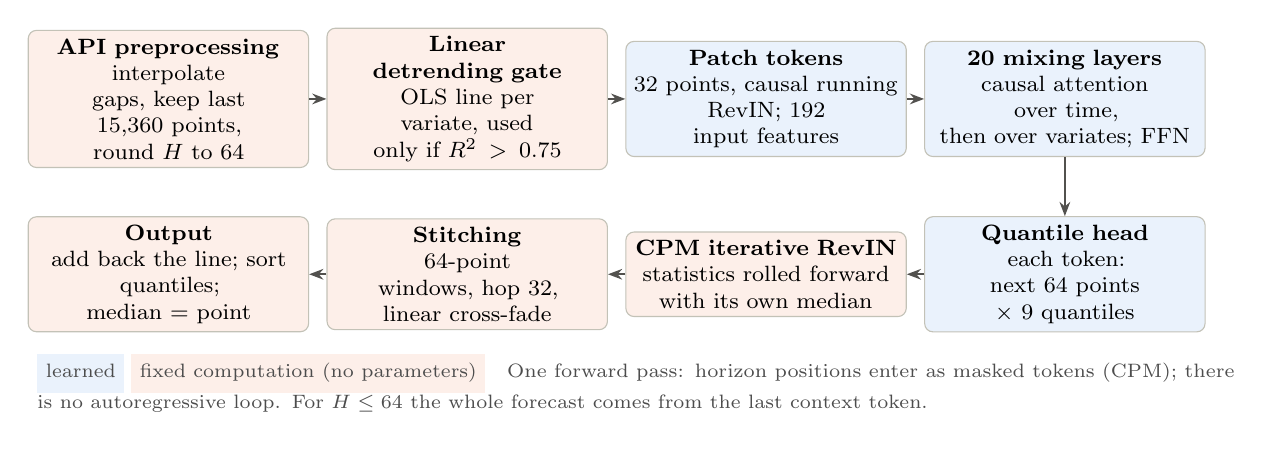
\begin{tikzpicture}[
  font=\footnotesize, node distance=0.22cm,
  blk/.style={draw=vzaxis, rounded corners=3pt, align=center, inner sep=3pt, text width=3.35cm, minimum height=1.05cm,
    execute at begin node={\hyphenpenalty=10000\exhyphenpenalty=10000}},
  fixed/.style={blk, fill=vzorangewash},
  learned/.style={blk, fill=vzbluewash},
  arr/.style={-{Stealth[length=1.8mm]}, thick, vzink2}
]
\node[fixed] (in) {\textbf{API preprocessing}\\ interpolate gaps, keep last\\ 15{,}360 points, round $H$ to 64};
\node[fixed, right=of in] (det) {\textbf{Linear detrending gate}\\ OLS line per variate, used\\ only if $R^2 > 0.75$};
\node[learned, right=of det] (tok) {\textbf{Patch tokens}\\ 32 points, causal running\\ RevIN; 192 input features};
\node[learned, right=of tok] (tr) {\textbf{20 mixing layers}\\ causal attention over time,\\ then over variates; FFN};
\node[learned, below=0.75cm of tr] (head) {\textbf{Quantile head}\\ each token: next 64 points\\ $\times$ 9 quantiles};
\node[fixed, left=of head] (cpm) {\textbf{CPM iterative RevIN}\\ statistics rolled forward\\ with its own median};
\node[fixed, left=of cpm] (st) {\textbf{Stitching}\\ 64-point windows, hop 32,\\ linear cross-fade};
\node[fixed, left=of st] (out) {\textbf{Output}\\ add back the line; sort\\ quantiles; median = point};
\draw[arr] (in) -- (det); \draw[arr] (det) -- (tok); \draw[arr] (tok) -- (tr); \draw[arr] (tr) -- (head);
\draw[arr] (head) -- (cpm); \draw[arr] (cpm) -- (st); \draw[arr] (st) -- (out);
\node[below=0.15cm of out.south west, anchor=north west, font=\scriptsize, text=black!70, text width=15.2cm]
  {\colorbox{vzbluewash}{\strut learned} \colorbox{vzorangewash}{\strut fixed computation (no parameters)}\quad
   One forward pass: horizon positions enter as masked tokens (CPM); there is no autoregressive loop.
   For $H \le 64$ the whole forecast comes from the last context token.};
\end{tikzpicture}
\caption{Inference path of TimesFM~3 as implemented in the public PyTorch code (\texttt{timesfm} 3.0.2), read line by line
(Section~\ref{sec:mechanism}). Shaded boxes are deterministic steps without parameters; four of them (detrending, CPM refinement,
stitching, quantile sorting) can shape a forecast, some only conditionally (the detrending gate; CPM and stitching only beyond 64
steps), but are not part of the network.}
\label{fig:architecture}
\end{figure}


\paragraph{Tokens and normalisation.} A series is cut into patches of 32 points aligned to its last observation; shorter batches
are left-padded with masked zeros, and the public API keeps at most the last 15{,}360 points. Each patch is normalised with the
mean and standard deviation of all observed points up to and including that patch (a causal, ``running'' RevIN), and the token
receives the 32 normalised values, a 64-point look-ahead channel and two mask channels (192 features), mapped to the model width
1{,}280 by a residual block. The look-ahead channel is non-empty only for covariates whose future values are known; for targets and
past-only covariates it is masked. Interior gaps are filled by linear interpolation before the model sees them: the network can take
point masks, but the forecasting API does not pass them, so missingness never reaches the model.

\paragraph{Transformer.} Twenty layers alternate, inside each layer, causal attention along the patch axis (rotary positions) and
full attention across variates at the same patch index, followed by a feed-forward block with no expansion (1{,}280 to 1{,}280);
the parameter count implied by the code shapes is about 330.7 million, as advertised. The checkpoint configuration sets
\texttt{use\_rope\_var = false}: attention across variates has no positional signal, so the model is equivariant to permutations of
the variates. A ``past-only covariate'' is encoded exactly as an extra target and is forecast and then discarded; inside the network
the two roles are indistinguishable. The limit of 32 variates mentioned in the documentation is not enforced by the model or by the
forecasting API; only the evaluator class used by Google's benchmark runners splits larger problems into chunks of 32 and randomly
subsamples covariates beyond that number.

\paragraph{Horizon and decoding.} Forecasting is a single forward pass. Every token predicts the next 64 points for nine quantiles
(0.1 to 0.9); the horizon is represented by masked tokens appended to the context (continuous patch masking, CPM). Overlapping
64-point windows of consecutive tokens, with a hop of 32, are cross-faded linearly (``stitching''). Because the statistics used to
de-normalise a horizon token cannot be observed, an iterative routine rolls them forward by treating the model's own median forecast
as if it were observed. Two consequences follow from the code. For horizons up to 64 steps, the entire forecast is produced by the
last context token, and neither the masked tokens nor the refinement play any role. With causal attention and no known future
covariates, the forecast of the first $h$ steps does not depend on the requested horizon.

\paragraph{Fixed computations around the network.} Four steps shape every forecast but have no parameters. (i) \emph{Linear
detrending:} each variate gets an ordinary least-squares line over its context, and the residuals are used instead of the series
when $\mathrm{std}(\text{residual}) < 0.5\,\mathrm{std}(\text{series})$, i.e.\ when the line explains more than 75\% of the
variance; the extrapolated line is then added back to all nine quantiles. The gate is discontinuous: a small change of the context
can switch it on or off. (ii) The CPM refinement described above. (iii) Stitching. (iv) Quantile sorting: the nine heads are
independent linear outputs, so they are sorted, and the point forecast is the fifth sorted value. Two further options are off by
default in the forecasting API but on in all of Google's benchmark runners: \emph{symmetric averaging}, which forecasts $x$ and $-x$
and averages the reflected quantiles (doubling the compute), and \emph{make positive}, which clips the quantiles of non-negative
series at zero. We call the package defaults \texttt{tfm3} and the runners' flags \texttt{tfm3-eval}.

\paragraph{Properties worth testing.} The design implies per-variate equivariance to positive affine transformations (each variate
is normalised by its own location and scale), equivariance to permutations of variates, no learned mechanism for missing data, and a
hard-coded linear extrapolation that may be harmful on saturating or regime-switching trends. Section~\ref{sec:controlled} tests the
last point (H3) and the ablations in Section~\ref{sec:ablations} switch each fixed step off in turn. The full reading of the code,
with line references, is released as \texttt{reports/mechanism.md}.

\section{Protocol}
\label{sec:protocol}

\begin{figure}[!htbp]
\centering
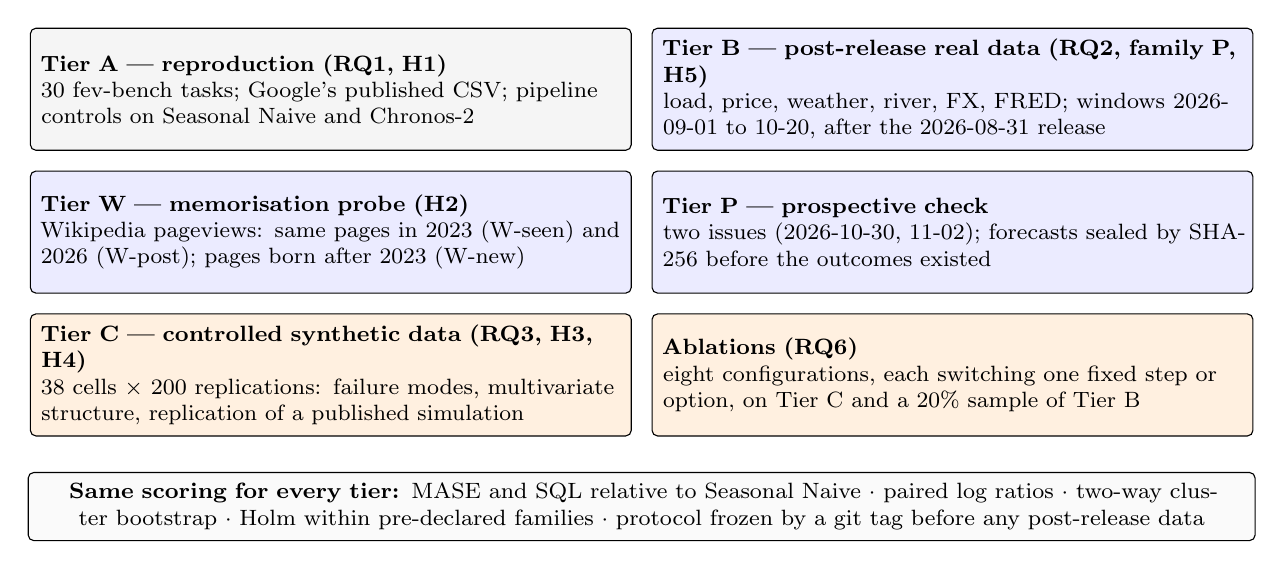
\begin{tikzpicture}[
  font=\footnotesize, node distance=0.25cm,
  tier/.style={draw, rounded corners=2pt, align=left, inner sep=4pt, text width=7.35cm, minimum height=1.55cm},
  arr/.style={-{Stealth[length=1.8mm]}, thick}
]
\node[tier, fill=black!4] (a) {\textbf{Tier A --- reproduction (RQ1, H1)}\\ 30 fev-bench tasks; Google's published CSV;
  pipeline controls on Seasonal Naive and Chronos-2};
\node[tier, fill=blue!8, right=of a] (b) {\textbf{Tier B --- post-release real data (RQ2, family P, H5)}\\ load, price, weather,
  river, FX, FRED; windows 2026-09-01 to 10-20, after the 2026-08-31 release};
\node[tier, fill=blue!8, below=of a] (w) {\textbf{Tier W --- memorisation probe (H2)}\\ Wikipedia pageviews: same pages in 2023
  (W-seen) and 2026 (W-post); pages born after 2023 (W-new)};
\node[tier, fill=blue!8, below=of b] (p) {\textbf{Tier P --- prospective check}\\ two issues (2026-10-30, 11-02); forecasts
  sealed by SHA-256 before the outcomes existed};
\node[tier, fill=orange!12, below=of w] (c) {\textbf{Tier C --- controlled synthetic data (RQ3, H3, H4)}\\ 38 cells $\times$ 200
  replications: failure modes, multivariate structure, replication of a published simulation};
\node[tier, fill=orange!12, below=of p] (abl) {\textbf{Ablations (RQ6)}\\ eight configurations, each switching one fixed step or
  option, on Tier C and a 20\% sample of Tier B};
\node[draw, rounded corners=2pt, fill=black!2, align=center, text width=15.3cm, inner sep=4pt, below=0.45cm of $(c.south)!0.5!(abl.south)$]
  (out) {\textbf{Same scoring for every tier:} MASE and SQL relative to Seasonal Naive $\cdot$ paired log ratios $\cdot$ two-way
  cluster bootstrap $\cdot$ Holm within pre-declared families $\cdot$ protocol frozen by a git tag before any post-release data};
\end{tikzpicture}
\caption{Study design. Tiers B and P, and the W-post and W-new strata of Tier W, use data published after TimesFM~3's release (blue; W-seen uses 2023 windows); Tier A is the public benchmark the
model was evaluated on, and Tier C and the ablations use synthetic data whose generating process is known (orange).}
\label{fig:design}
\end{figure}

\begin{figure}[!t]
\centering
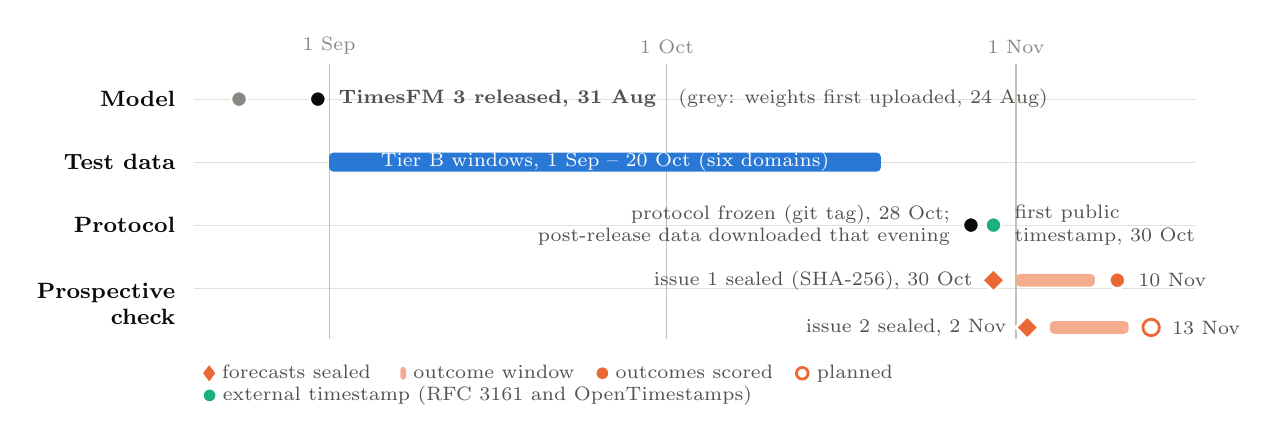
\begin{tikzpicture}[x=0.143cm, y=1cm, font=\footnotesize,
  lane/.style={font=\footnotesize\bfseries, text=vzink, anchor=east},
  ev/.style={circle, fill=#1, draw=white, line width=1pt, inner sep=2.1pt},
  seal/.style={diamond, fill=#1, draw=white, line width=1pt, inner sep=2.2pt},
  lab/.style={font=\scriptsize, text=vzink2, align=#1},
  band/.style={fill=#1, rounded corners=1.5pt}]
% day 0 = 2026-08-20
\foreach \y in {0,-0.8,-1.6,-2.4} \draw[vzgrid, line width=0.4pt] (0,\y) -- (89,\y);
\foreach \d/\m in {12/1 Sep, 42/1 Oct, 73/1 Nov} {
  \draw[vzaxis, line width=0.4pt] (\d,0.45) -- (\d,-3.05);
  \node[font=\scriptsize, text=vzmuted, anchor=south] at (\d,0.45) {\m};}
\node[lane] at (-0.8,0) {Model};
\node[lane] at (-0.8,-0.8) {Test data};
\node[lane] at (-0.8,-1.6) {Protocol};
\node[lane, align=right] at (-0.8,-2.6) {Prospective\\check};
% model
\node[ev=vzmuted] (w) at (4,0) {};
\node[ev=vzink] (r) at (11,0) {};
\node[lab=left, anchor=west] at (12,0) {\textbf{TimesFM~3 released, 31 Aug}\quad (grey: weights first uploaded, 24 Aug)};
% Tier B windows
\fill[band=vzblue] (12,-0.92) rectangle (61,-0.68);
\node[font=\scriptsize, text=white, anchor=center] at (36.5,-0.8) {Tier B windows, 1 Sep -- 20 Oct (six domains)};
% protocol
\node[ev=vzink] (f) at (69,-1.6) {};
\node[lab=right, anchor=east] at (68,-1.6) {protocol frozen (git tag), 28 Oct;\\post-release data downloaded that evening};
\node[ev=vzaqua] at (71,-1.6) {};
\node[lab=left, anchor=west] at (72,-1.6) {first public\\timestamp, 30 Oct};
% prospective issues
\node[seal=vzorange] at (71,-2.3) {};
\fill[band=vzorange!55] (73,-2.38) rectangle (80,-2.22);
\node[ev=vzorange] at (82,-2.3) {};
\node[lab=right, anchor=east] at (70,-2.3) {issue 1 sealed (SHA-256), 30 Oct};
\node[lab=left, anchor=west] at (83,-2.3) {10 Nov};
\node[seal=vzorange] at (74,-2.9) {};
\fill[band=vzorange!55] (76,-2.98) rectangle (83,-2.82);
\node[circle, fill=white, draw=vzorange, line width=1pt, inner sep=2.1pt] at (85,-2.9) {}; % planned: switch to ev=vzorange once scored
\node[lab=right, anchor=east] at (73,-2.9) {issue 2 sealed, 2 Nov};
\node[lab=left, anchor=west] at (86,-2.9) {13 Nov};
% legend
\node[font=\scriptsize, text=vzink2, anchor=north west, align=left] at (0,-3.25)
  {\tikz[baseline=-0.6ex]{\pgfsetfillcolor{vzorange}\pgfsetstrokecolor{vzorange}\pgfsetplotmarksize{2.6pt}\pgfuseplotmark{diamond*}}~forecasts sealed \quad
   \tikz[baseline=-0.6ex]\fill[vzorange!55, rounded corners=1pt] (0,-0.08) rectangle (0.5,0.08);~outcome window\quad
   \tikz[baseline=-0.6ex]\fill[vzorange] (0,0) circle (2.1pt);~outcomes scored\quad
   \tikz[baseline=-0.6ex]\draw[vzorange, line width=1pt] (0,0) circle (2.1pt);~planned\\
   \tikz[baseline=-0.6ex]\fill[vzaqua] (0,0) circle (2.1pt);~external timestamp (RFC~3161 and OpenTimestamps)};
\end{tikzpicture}
\caption{Chronology, 2026. Every Tier B test window starts after TimesFM~3's release; the protocol was frozen by a git tag
before the post-release data were downloaded (an internal record; its first external timestamp is two days later); the two
prospective issues were sealed by hash before their outcomes existed and are scored after the outcome windows close.}
\label{fig:timeline}
\end{figure}


\paragraph{Freeze.} Research questions, hypotheses, series lists, metrics, contrasts, families and decision rules were written in a
protocol and frozen by the git tag \texttt{protocol-frozen-v1} (commit \texttt{9f15b38}, 2026-10-28 17:59 UTC) before any data of
the post-release test windows were downloaded; the download code refuses earlier dates. The freeze is internal: the hash of the
frozen commit received its first public timestamp on 2026-10-30, after the download, so the order of freeze and download rests
on the repository history, not on an external record (Figure~\ref{fig:timeline}). The protocol incorporates an independent
adversarial review of its draft and a pilot on pre-release data (one year earlier) and on a separate synthetic set; the pilot is not
part of the results. Two deviations occurred (Appendix~\ref{app:deviations}): the post-release data were downloaded on the evening of
the freeze day instead of the next day, and a software error voided one ablation, which was re-run. Interpretations of
ambiguous protocol items are listed with them. Results that the protocol did not specify are labelled \emph{exploratory} or
\emph{descriptive} wherever they appear.

\paragraph{Research questions.} RQ1: do the published per-task TimesFM~3 results, and the claim they support, reproduce with the
public code and weights? RQ2: does TimesFM~3's advantage hold on data that post-date its release, and is there a trace of
memorisation? RQ3: under which controlled conditions does zero-shot forecasting fail? RQ4: are the quantile forecasts calibrated?
RQ5: when do multivariate mode and covariates help? RQ6: how much do inference-time options and fixed components contribute? RQ7: is
zero-shot forecasting worth it against classical methods, accounting for compute?

\paragraph{Pre-declared hypotheses.} \textbf{H1} (descriptive): the advantage over a statistical ensemble is smaller on post-release
data than on the public benchmark. \textbf{H2}: on Wikipedia pageviews, TimesFM~3's advantage over Chronos-2 is larger on
2023 windows inside TimesFM's pageview corpus (W-seen) than on the same pages in 2026 (W-post). \textbf{H3}: disabling the linear
detrending lowers the error over steps 25--48 on a saturating logistic process. \textbf{H4}: multivariate mode lowers the error
when a known dependence exists (H4a lead-lag, H4b known future covariate) and is equivalent within $\pm$3\% when none exists (H4c
independent series, H4d spurious covariate). \textbf{H5}: on near-random-walk series (exchange rates, Treasury yields, oil prices)
TimesFM~3 does not improve on the random walk by more than 10\%.

\paragraph{Metrics.} The point metric is MASE of the median forecast and the probabilistic metric is the scaled quantile loss (SQL)
over the nine quantile levels, both as defined by fev-bench \citep{shchur2025fevbench}; scales are the in-sample seasonal
differences of each task's full context (season 24 for hourly, 7 for daily, 5 for business-daily data), the same for every model
whatever context it is given, so the scale cancels in a paired ratio. We also record RMSSE, WAPE, WQL and the
empirical coverage of the 80\% and 60\% central intervals.

\paragraph{Estimand and uncertainty.} A contrast between configurations A and B is the paired log ratio
$d = \log(\text{error}_A) - \log(\text{error}_B)$ on identical series and windows, averaged with equal weight within each domain
$\times$ horizon cell, then over horizons and over domains, and reported as $\exp(\bar d)$: a ratio below 1 favours A. Uncertainty
comes from a two-way cluster bootstrap with 10{,}000 replicates that resamples series (within domains) and ISO weeks of the first
forecast step jointly \citep{cameron2011multiway}: each replicate draws multinomial weights for series and for weeks and multiplies them
(a pigeonhole bootstrap, \citealp{owen2007pigeonhole}), so the dependence within a series and the shocks common to several series in the same week are reflected.
Dependence between different series in different but overlapping windows is not, and with eight weekly clusters temporal
inference is weak (Section~\ref{sec:robustness}). Synthetic data resample replications. Pairs where either error is zero or not
finite are dropped (the log ratio is undefined). Intervals are percentile 95\% intervals; $p$-values are two-sided, twice the smaller share of replicates on either side
of zero, with a floor of $1/10{,}000$ (seed 17); the series-only interval is reported as a sensitivity analysis.

\paragraph{Families and decisions.} Decisions use Holm-adjusted $p$-values \citep{holm1979} within a family at
$\alpha = 0.05$; intervals are unadjusted. \emph{Family P} (primary, ten tests) holds five contrasts on
post-release data, each on MASE and SQL: TimesFM~3 in univariate mode without covariates against the statistical ensemble (P1),
Chronos-2 (P2) and TimesFM~2.5 (P3), all without covariates, on the same 3{,}855 univariate evaluations of the four structured
domains (on hourly data the context lengths differ; Section~\ref{sec:data}); the multivariate against the univariate mode on the
884 evaluations of the price, FX and FRED group tasks, which have no covariates (P4a); and the benchmark flags against the package
defaults on the 3{,}855 univariate evaluations, both configurations with the covariates of load and river flow (P5). \emph{Family H} holds the primary test of each hypothesis H2--H5
(seven tests). Equivalence (H4c, H4d) is claimed only if the 90\% interval lies inside the $\pm$3\% margin (two one-sided tests
\citep{schuirmann1987tost}); H5 is a non-superiority test that is supported when the 95\% lower bound exceeds 0.90. A
difference whose adjusted $p$ exceeds 0.05 is reported as \emph{not resolved}, never as a tie. Secondary families (S1--S6) have their
own Holm correction.

\section{Data and models}
\label{sec:data}

\paragraph{Tier A: public benchmark.} Thirty of the 100 fev-bench tasks \citep{shchur2025fevbench}, sampled with a fixed seed and
stratified by domain and frequency, after excluding the three tasks whose string covariates Google's runner encodes with Python's
salted \texttt{hash()} (not reproducible across processes). Metrics are computed with fev's own functions, and every Tier A model uses
the conventions of Google's runner (last-value imputation, context cut to 15{,}360 points). Two pipeline controls are required on
every task: our Seasonal Naive must match fev's published results ($|\Delta\mathrm{MASE}| < 5\cdot10^{-5}$) and our Chronos-2 fev's
published Chronos-2 ($|\Delta\mathrm{SQL}| \le 0.5\%$).

\paragraph{Tier B: post-release real data.} TimesFM~3 was released on 2026-08-31. The test windows run from 2026-09-01 to
2026-10-20, with origins every 24 hours for 24-hour horizons and weekly otherwise (168 hours, 7 days or 5 business days). Six domains, with
series lists fixed by rules on 2025 data: hourly electricity load in 12 European countries and day-ahead prices in 12 bidding zones
(Energy-Charts \citep{energycharts2026}), hourly temperature and wind speed in 20 cities (ERA5 via Open-Meteo
\citep{hersbach2020era5,zippenfenig2023openmeteo}), daily flow at 20 river gauges (USGS \citep{usgs2026nwis}), ten business-daily exchange rates
against the euro (ECB \citep{ecb2026dataportal}), and eight Treasury yields with WTI and Brent prices (FRED \citep{fred2026}). Horizons are 24 and
168 hours, 7 and 28 days, 5 and 20 business days. Load and river flow have a covariate whose \emph{observed} future values are
supplied (temperature, precipitation): it is an oracle, used only in secondary analyses as an upper bound. Price, FX and FRED also
form one group task each, in which all series of the domain are forecast jointly. Same-source data of earlier periods are part of
the public pre-training corpora for load, price and weather; the model card describes the TimesFM~3 corpus only at the level of sources (GiftEvalPretrain without the
datasets that overlap fev-bench, Wikipedia pageviews to November 2023, Google Trends to 2022, synthetic data
\citep{timesfm2026hf}), so Tier B guarantees
that the \emph{test windows} are new, not that the series are.

\paragraph{Tier W: memorisation probe.} English Wikipedia daily user pageviews \citep{wikimedia2026pageviews}, horizons 7 and 28 days,
400-day contexts. \emph{W-seen}: 200 popular pages (seed 17) with test windows from 2023-09-01 to 2023-10-20, inside the pageview
corpus that the TimesFM~3 model card lists up to November 2023 \citep{timesfm2026hf}. \emph{W-post}: the same pages, same calendar span in
2026. \emph{W-new}: pages that first entered the top-1000 lists in 2024--2025, with no views at all before December 2023, matched to
W-seen/W-post on quintiles of median views. Pages that became redirects are excluded (190 and 128 pages remain).

\paragraph{Tier C: controlled synthetic data.} 38 cells with 200 replications each (7{,}600 tasks), seeded per cell and
replication: (i) a replication of the three hard processes of a recent simulation study of zero-shot forecasting
\citep{ebrahim2026foundation}, level shift (D6), logistic growth (D7) and intermittent demand (D8), with contexts of 48 and 200 points and
horizons 12 and 48; (ii) univariate stress cells: two seasonalities with one or four weeks of context, a season longer than the
context, a context ladder from 64 to 15{,}360 points, horizons up to 1{,}024, a regime change near the origin, outliers in the last
5\% of the context, a random walk and white noise; (iii) multivariate cells: VAR(1) systems of 2 to 64 variates, lead-lag pairs
(lags 1, 5, 24), a target driven by a known future covariate (signal-to-noise 0.5 and 2), a spurious past covariate, and independent
series stacked as variates.

\paragraph{Tier P: prospective check.} On the morning of each issue day (2026-10-30 and 2026-11-02) the data published up to the
previous day are downloaded for the load, price, river, FX, FRED and Wikipedia series, every series is forecast from its last
observation, and the contexts, tasks, code bundle, run records and forecast files are hashed together; the combined SHA-256 is
recorded before the scoring window (from two to nine days after the issue day) starts.

\paragraph{Models.} Table~\ref{tab:models} lists the configurations. Every Hugging Face model is loaded by revision hash.
TimesFM~3 runs in four configurations: package defaults in multivariate mode with covariates (\texttt{tfm3}), univariate without
covariates (\texttt{tfm3-uni}, the configuration of the information-matched contrasts), the flags of Google's benchmark runners
(\texttt{tfm3-eval}), and univariate with the classical models' context of 2{,}016 points (\texttt{tfm3-c2016}). The comparison
foundation models are TimesFM~2.5 \citep{das2024timesfm}, Chronos-2 \citep{ansari2025chronos2} and TiRex-2 \citep{podest2026tirex2}, each also
in a univariate configuration where relevant. The classical models are StatsForecast \citep{garza2022statsforecast} implementations of
AutoETS, AutoARIMA and AutoTheta, MSTL with seasons 24 and 168 \citep{bandara2025mstl} for hourly data, and Naive, Seasonal Naive and
the historic mean. Classical models use at most the last 2{,}016 hourly, 1{,}095 daily or 780 business-daily observations,
the foundation models up to 15{,}360 (Chronos-2 truncates at 8{,}192). On daily and business-daily data all models therefore see the
same history; on hourly data the foundation models see about 15{,}000 points, and \texttt{tfm3-c2016} measures the effect of that
difference for TimesFM~3. The statistical ensemble averages the quantiles of three members: MSTL with ETS, Theta and ARIMA remainders on
hourly data, and AutoETS, AutoARIMA and AutoTheta otherwise. All foundation models ran on a free Google Colab Tesla T4 GPU in fp32;
classical models ran on eight cores of a local CPU.

\begin{table}[!htbp]
\centering
\caption{Model configurations.}
\label{tab:models}
\scriptsize
\begin{tabular}{llp{7.6cm}}
\toprule
Key & Model (revision) & Configuration \\
\midrule
\texttt{tfm3} & TimesFM~3, 330M (\texttt{43046b85}) & package defaults; all targets and covariates of a task in one pass \\
\texttt{tfm3-uni} & TimesFM~3 & package defaults; each target alone, no covariates \\
\texttt{tfm3-eval} & TimesFM~3 & as \texttt{tfm3} with symmetric averaging and \emph{make positive} \\
\texttt{tfm3-c2016} & TimesFM~3 & as \texttt{tfm3-uni}, last 2{,}016 points only \\
\texttt{tfm25} & TimesFM~2.5, 200M (\texttt{1d952420}) & univariate, recommended flags \\
\texttt{chronos2}, \texttt{-uni} & Chronos-2, 120M (\texttt{29ec3766}) & \texttt{predict\_df}; with / without covariates and joint targets \\
\texttt{tirex2}, \texttt{-uni} & TiRex-2 (\texttt{30788a31}) & as Chronos-2; horizons up to 320 \\
\texttt{stat-ens} & equal-weight ensemble & MSTL-\{ETS, Theta, ARIMA\} (hourly); AutoETS, AutoARIMA, AutoTheta \\
classical & StatsForecast 2.1.1 & Naive, Seasonal Naive, mean, AutoETS, AutoARIMA, AutoTheta, MSTL variants \\
\bottomrule
\end{tabular}
\end{table}

\section{Results I: the published results reproduce}
\label{sec:reproduction}

\paragraph{Per-task reproduction (RQ1).} With the benchmark flags (\texttt{tfm3-eval}), our SQL is within $\pm$3\% of Google's
published value on \AReproShare\% of the \ATasks{} tasks we could score (Table~\ref{tab:tiera}); the median deviation is zero to four
decimals and the deviations show no systematic sign. The two remaining tasks of the sample (\texttt{boomlet\_619},
\texttt{boomlet\_1209}) exhaust the 15\,GB of the T4 GPU under symmetric averaging, which doubles the batch, and are not scored;
the package defaults (\texttt{tfm3}) run on all 30. The five tasks outside the $\pm$3\% band (deviations from $-10.6\%$ to
$+6.1\%$; four of the five in our favour) all have covariates: the median absolute deviation is 0.001\% on tasks without covariates
and 1\% on tasks with covariates. We did not trace the cause; candidates are the handling of covariates with missing values and
batch-size choices that depend on the hardware. The per-task values are in Appendix~\ref{app:tiera}.

\begin{table}[!htbp]
\centering
\caption{Tier A: reproduction of Google's published fev-bench results. ``$\pm$3\%'': share of tasks whose SQL is within 3\%
of the published value; ``Median'' and ``Range'': deviations relative to the published SQL. ``Ratio'': geometric mean over tasks of SQL(TimesFM~3) /
SQL(Chronos-2), with our Chronos-2 (``ours'', no cross-learning) or fev's published Chronos-2 (``publ.'', cross-learning).}
\label{tab:tiera}
\scriptsize
\setlength{\tabcolsep}{3.5pt}
\begin{tabular}{llrrrlrr}
\toprule
Model & Tasks & $n$ & $\pm$3\% & Median & Range & Ratio ours & Ratio publ. \\
\midrule
TimesFM-3 eval & all tasks & 28 & 82\% & 0.00\% & [-10.6\%, +6.1\%] & 0.954 & 0.973 \\
TimesFM-3 eval & tasks passing both controls & 10 & 90\% & 0.00\% & [-0.4\%, +6.1\%] & 1.004 & 0.997 \\
TimesFM-3 & all tasks & 30 & 77\% & +0.24\% & [-8.9\%, +29.9\%] & 0.970 & 0.972 \\
TimesFM-3 & tasks passing both controls & 12 & 75\% & +0.55\% & [-0.3\%, +29.9\%] & 1.027 & 0.990 \\
\bottomrule
\end{tabular}

\end{table}

\paragraph{The claim against Chronos-2.} Google's comparison sets its TimesFM~3 results against the Chronos-2 results published by
fev. Our Chronos-2 failed the pipeline control on 16 of the 28 tasks (two further tasks failed the Seasonal Naive control), with a
higher SQL than published on 12 of them, so we traced the cause. fev's
published Chronos-2 results were produced with \emph{cross-learning} switched on: the series of a batch of up to 100 share
information through Chronos-2's group attention. Running fev's own evaluation script on five failing tasks reproduces the published
SQL to a relative difference of $4\cdot10^{-6}$ with cross-learning on and our values with it off (Appendix~\ref{app:chronos}); input preparation (batching,
imputation, timestamps) changes nothing. TimesFM~3 has no comparable option: it forecasts each series of a task on its own, or the
series of one multivariate task jointly. Cross-learning lowered Chronos-2's SQL by 2--9\% on four of the five tasks and raised it by
11\% on the fifth. With both models forecasting each series on its own, the geometric-mean SQL ratio of TimesFM~3 to Chronos-2 is
\ASkillOurs{} on all scored tasks, against \ASkillPubl{} in the published comparison: without cross-learning on the Chronos-2 side,
TimesFM~3's lead is slightly larger, not smaller. The lead comes from the \AFailTasks{} tasks where the controls fail
(\ASkillOursFail{} ours, \ASkillPublFail{} published); on the \AControlTasks{} tasks where our Chronos-2 matches fev's, the two
models are at parity in both comparisons (\ASkillOursCtl{} and \ASkillPublCtl{}). The published claim therefore holds on this
sample; what a leaderboard does not show is that the two result sets were produced with different inference options, one of which
favours Chronos-2 on most of the tasks it affects.

\paragraph{Against classical methods (H1, Tier A side).} With Google's inputs, TimesFM~3 (\texttt{tfm3}) has a geometric-mean
MASE of \HoneAMase{} and SQL of \HoneASql{} relative to fev's published statistical ensemble over the \HoneATasks{} tasks for which fev reports the ensemble, and a lower
SQL on \HoneAWins\% of them. Section~\ref{sec:postrelease} sets these numbers against the same comparison on post-release data.

\section{Results II: post-release data}
\label{sec:postrelease}

\begin{figure}[!htbp]
\centering
\pgfplotstableread{
x y em ep fam res
1.1096 0 0.0608 0.0688 1 1
1.0004 1 0.0006 0.0006 1 1
0.9979 2 0.0013 0.0013 1 1
0.4458 3 0.0143 0.0145 1 1
0.6159 4 0.0247 0.0266 1 1
0.9799 5 0.0438 0.0408 1 0
0.9894 6 0.0133 0.0125 0 0
0.9667 7 0.0266 0.0300 0 0
0.9509 8 0.0334 0.0372 0 0
0.9528 9 0.0290 0.0280 0 1
0.8358 10 0.0502 0.0462 0 1
}\forestdata
\pgfplotsset{forest ticks/.style={ytick={0,1,2,3,4,5,6,7,8,9,10}, yticklabels={{H5: TimesFM-3 uni vs Naive, FX and FRED},{H4d: multivariate vs univariate, spurious covariate},{H4c: multivariate vs univariate, independent series},{H4b: multivariate vs univariate, known covariate},{H4a: multivariate vs univariate, lead-lag 24},{H2: W-seen vs W-post DiD, TimesFM-3 vs Chronos-2},{P5: TimesFM-3 eval vs TimesFM-3},{P4a: TimesFM-3 vs TimesFM-3 uni},{P3: TimesFM-3 uni vs TimesFM-2.5},{P2: TimesFM-3 uni vs Chronos-2 uni},{P1: TimesFM-3 uni vs Stat.\ ensemble}}, ymin=-0.7, ymax=10.7}}

\begin{tikzpicture}
\begin{axis}[
  width=0.62\textwidth, height=9.2cm,
  xmode=log, log basis x=10, xmin=0.4, xmax=1.3,
  xtick={0.5,0.6,0.7,0.8,0.9,1,1.1,1.2}, xticklabels={0.5,0.6,0.7,0.8,0.9,1,1.1,1.2},
  forest ticks, yticklabel style={font=\scriptsize, align=right},
  xlabel={ratio of errors, A / B (log scale; $<1$: A better)}, xlabel style={font=\footnotesize},
  tick label style={font=\footnotesize},
  axis lines*=left, ymajorgrids=false, xmajorgrids=true, grid style={black!10},
  clip=false]
\addplot[black!40, dashed] coordinates {(1,-0.7) (1,10.7)};
\addplot[only marks, mark=*, mark size=1.6pt, black,
  error bars/.cd, x dir=both, x explicit, error bar style={line width=0.8pt}]
  table[x=x, y=y, x error minus=em, x error plus=ep] {\forestdata};
\end{axis}
\end{tikzpicture}
\caption{Primary (family P, MASE) and hypothesis (family H) contrasts: estimate and two-way cluster bootstrap 95\% interval
(unadjusted). P-tests are on post-release Tier B data: P1--P3 without covariates on the same series and windows (context lengths differ on
hourly data), P4a on the group tasks (no covariates), P5 between two configurations with the covariates of load and river flow; H4a--H4d are on controlled
multivariate data; H5 is on exchange rates, Treasury yields and oil prices. H3 is omitted (its cell never activates the mechanism
it tests, Section~\ref{sec:controlled}). Decisions use Holm-adjusted $p$-values (Tables~\ref{tab:familyp} and~\ref{tab:familyh}).}
\label{fig:forest}
\end{figure}


\paragraph{Primary contrasts (family P).} On the four structured domains of Tier B, with no covariates for any model, TimesFM~3 in
univariate mode has a MASE \PoneMase{} times that of the statistical ensemble (95\% CI \PoneMaseLo--\PoneMaseHi) and an SQL
\PoneSql{} times (\PoneSqlLo--\PoneSqlHi); both differences are resolved (Table~\ref{tab:familyp}, Figure~\ref{fig:forest}). Against
the other foundation models the margins are an order of magnitude smaller: \PtwoMase{} (MASE) and \PtwoSql{} (SQL) against
Chronos-2, both resolved, and \PthreeSql{} (SQL, resolved) and \PthreeMase{} (MASE, not resolved after Holm correction) against its
predecessor TimesFM~2.5. Joint forecasting of the real group tasks (P4a: price, FX, FRED) lowers SQL by about 3\% (resolved; the
MASE difference is not resolved). The flags of Google's benchmark runners (P5) change neither metric by more than about 1\%, at
twice the compute; neither difference is resolved.

\begin{table}[!htbp]
\centering
\caption{Family P (primary): information-matched contrasts on Tier B. Ratio of errors, A / B ($<1$: A better), with the
two-way cluster bootstrap interval and the series-only interval; decisions by Holm-adjusted $p$ over the ten tests.}
\label{tab:familyp}
\scriptsize
\setlength{\tabcolsep}{4pt}
\begin{tabular}{lllrllll}
\toprule
Test & Contrast (A vs B) & Metric & Ratio & 95\% CI (two-way) & 95\% CI (series) & $p_{\mathrm{Holm}}$ & Decision \\
\midrule
P1 & TimesFM-3 uni vs Stat.\ ensemble & MASE & 0.836 & [0.786, 0.882] & [0.804, 0.867] & 0.001 & resolved \\
P1 & TimesFM-3 uni vs Stat.\ ensemble & SQL & 0.707 & [0.649, 0.764] & [0.655, 0.757] & 0.001 & resolved \\
P2 & TimesFM-3 uni vs Chronos-2 uni & MASE & 0.953 & [0.924, 0.981] & [0.937, 0.969] & 0.014 & resolved \\
P2 & TimesFM-3 uni vs Chronos-2 uni & SQL & 0.956 & [0.933, 0.979] & [0.942, 0.971] & 0.003 & resolved \\
P3 & TimesFM-3 uni vs TimesFM-2.5 & MASE & 0.951 & [0.917, 0.988] & [0.924, 0.981] & 0.066 & not resolved \\
P3 & TimesFM-3 uni vs TimesFM-2.5 & SQL & 0.939 & [0.914, 0.965] & [0.916, 0.963] & 0.001 & resolved \\
P4a & TimesFM-3 vs TimesFM-3 uni & MASE & 0.967 & [0.940, 0.997] & [0.947, 0.986] & 0.105 & not resolved \\
P4a & TimesFM-3 vs TimesFM-3 uni & SQL & 0.966 & [0.947, 0.988] & [0.950, 0.982] & 0.025 & resolved \\
P5 & TimesFM-3 eval vs TimesFM-3 & MASE & 0.989 & [0.976, 1.002] & [0.983, 0.995] & 0.106 & not resolved \\
P5 & TimesFM-3 eval vs TimesFM-3 & SQL & 0.991 & [0.982, 1.000] & [0.986, 0.996] & 0.106 & not resolved \\
\bottomrule
\end{tabular}

\end{table}

\paragraph{By domain (S1).} The advantage over the statistical ensemble is resolved in every domain, from 11\% lower MASE on
electricity load to 22\% on river flow (Table~\ref{tab:secondary}). Against Chronos-2 the per-domain differences are resolved only
on weather; against TimesFM~2.5 on load and weather. The cross-model margins are therefore not uniform across domains, and the
pooled P2 result rests mostly on the largest domain (weather: 2{,}280 of 3{,}855 series-windows).

\paragraph{H1: is the advantage smaller after the release?} With the same configuration as on Tier A (package defaults, covariates
included), TimesFM~3's MASE relative to our statistical ensemble on Tier B is \HoneBMase{} (\HoneBMaseLo--\HoneBMaseHi) and its SQL
\HoneBSql{} (\HoneBSqlLo--\HoneBSqlHi), against \HoneAMase{} and \HoneASql{} relative to fev's ensemble on the benchmark tasks.
Descriptively, the point-forecast advantage is about a quarter smaller on post-release data (18\% against 25\%) and the
probabilistic advantage almost unchanged (31\% against 34\%). The two tiers differ in datasets, horizons and ensemble members, so
this comparison carries no test and cannot separate exposure from difficulty; it says that the benchmark-level advantage over
classical methods survives on new data, slightly reduced for the median forecast.

\paragraph{H5: near-random-walk series.} On exchange rates, Treasury yields and oil prices, TimesFM~3's MASE is \Hfive{} times that
of the random walk (\HfiveLo--\HfiveHi): H5 is supported, and more strongly than stated, since the model is \emph{worse} than the
naive forecast rather than not much better. It is also worse than the statistical ensemble on these series (\NrwStatEns,
\NrwStatEnsLo--\NrwStatEnsHi; descriptive), while the difference from Chronos-2 is not resolved (\NrwChronos,
\NrwChronosLo--\NrwChronosHi). A random walk is the optimal forecast for a martingale, so no model can beat it by a resolved margin
without an evaluation problem; the negative controls in Tier C behave the same way (Section~\ref{sec:controlled}).

\paragraph{Covariates and context length (S3, S4).} Supplying the observed future temperature for load and the observed future
precipitation for river flow, an oracle that no real forecast has, does not resolve a gain: \texttt{tfm3} against \texttt{tfm3-uni}
gives 0.974 (0.904--1.060), and Chronos-2 with and without covariates 0.969 (0.930--1.008). On hourly data, cutting TimesFM~3's
context to the 2{,}016 points the classical models use raises its MASE by 4\% (S4, resolved); the long context helps, but explains
only a small part of the gap to the classical ensemble on hourly series (11--13\% in load and price).

\paragraph{Memorisation probe (H2, S2).} TimesFM~3's MASE relative to Chronos-2 is 0.939 on the 2023 W-seen windows and 0.959 on the
same pages in 2026; the difference in differences is \Htwo{} (\HtwoLo--\HtwoHi), not resolved (Table~\ref{tab:familyh}). The design
had 80\% power to detect a difference of about 5\%, so a memorisation advantage of that size is unlikely; smaller effects cannot be
excluded, and a null difference does not show that the pages were not memorised. The secondary contrasts agree
(Table~\ref{tab:secondary}): with the statistical ensemble or TiRex-2 as the reference, and for TimesFM~2.5, the difference is not
resolved. On pages born after 2023 (W-new), TimesFM~3's advantage over Chronos-2 is smaller than on W-post (0.984 against 0.959); the
raw contrast is not resolved, and the contrast adjusted for context features (0.942, 0.897--0.996) is not resolved after Holm
correction. If anything, TimesFM~3 does slightly better on long-lived pages than on new ones, which is consistent with familiarity
with the type of series rather than with the particular windows.

\paragraph{Calibration (RQ4).} The empirical coverage of the nominal 80\% interval on Tier B is close to nominal for TimesFM~3
(\CovBtfm{}), TimesFM~2.5 and TiRex-2, lower for Chronos-2 (0.750) and lower for the statistical ensemble (\CovBstat{}), whose MSTL
intervals ignore the uncertainty of the seasonal component (Table~\ref{tab:calibration}). On Wikipedia pageviews all foundation
models are too narrow (coverage 0.72--0.76) and the ensemble far too wide (0.95). The Wilson intervals use the number of series as the sample size and are therefore wide; they are a guide,
not a test.

\paragraph{Exploratory: spikes and lineage.} These analyses were declared exploratory (protocol §5.3) and are not corrected for
multiplicity. (i) \emph{Spike anticipation on W.} In 191 of the 5{,}588 Wikipedia windows the observed maximum exceeds three times
the 90th percentile of the context. In the 161 of them where the spike starts after the forecast origin, no foundation model
anticipates it: the maximum of TimesFM~3's 0.9 quantile over the window has a median of 1.09 times the context percentile (observed:
4.7), and exceeds three times the percentile in 9\% of these windows (Chronos-2 8\%, TiRex-2 and TimesFM~2.5 3\%). The naive
forecast reaches that level more often (48\%) only because its intervals widen with the horizon. In the 30 windows where the spike is
already under way at the origin, all foundation models extend it. The share does not differ between W-seen and W-post for TimesFM~3
(0.189 and 0.191), which agrees with the memorisation probe. (ii) \emph{Lineage.} On the structured domains of Tier B,
TimesFM~3's MASE relative to the statistical ensemble is 0.857 (0.823--0.889) on series whose source has earlier-period data in
public pre-training corpora (load, price, weather) and 0.776 (0.636--0.922) on rivers, for which none is known. The advantage is not
larger where exposure to the source is documented; since the lineage groups coincide with domains, this is not a test of exposure.

\begin{table}[!htbp]
\centering
\caption{Calibration: mean empirical coverage of the central 80\% and 60\% intervals (protocol §5.6). The Wilson interval treats
each series as one observation (each series' coverage averaged over its windows and steps).}
\label{tab:calibration}
\small
\begin{tabular}{lrrr}
\toprule
Model & Series & Coverage 80\% & Coverage 60\% \\
\midrule
\multicolumn{4}{l}{\textit{Tier B (structured, univariate tasks)}} \\
TimesFM-3 uni & 84 & 0.796 & 0.596 \\
TimesFM-3 & 84 & 0.802 & 0.598 \\
TimesFM-3 eval & 84 & 0.807 & 0.604 \\
TimesFM-2.5 & 84 & 0.807 & 0.607 \\
Chronos-2 uni & 84 & 0.750 & 0.546 \\
TiRex-2 uni & 84 & 0.797 & 0.599 \\
Stat.\ ensemble & 84 & 0.779 & 0.630 \\
\multicolumn{4}{l}{\textit{Tier W, W-post}} \\
TimesFM-3 & 190 & 0.761 & 0.553 \\
TimesFM-2.5 & 190 & 0.755 & 0.563 \\
Chronos-2 & 190 & 0.722 & 0.520 \\
TiRex-2 & 190 & 0.760 & 0.560 \\
Stat.\ ensemble & 190 & 0.946 & 0.886 \\
\multicolumn{4}{l}{\textit{Tier C (all cells)}} \\
TimesFM-3 & 7600 & 0.807 & 0.597 \\
TimesFM-2.5 & 7600 & 0.804 & 0.616 \\
Chronos-2 & 7600 & 0.780 & 0.544 \\
TiRex-2 & 7200 & 0.821 & 0.635 \\
Stat.\ ensemble & 7600 & 0.866 & 0.728 \\
\multicolumn{4}{l}{\textit{Tier P, both issues: load, price, river}} \\
TimesFM-3 uni & 44 & 0.699 & --- \\
TimesFM-2.5 & 44 & 0.707 & --- \\
Chronos-2 uni & 44 & 0.672 & --- \\
TiRex-2 uni & 44 & 0.732 & --- \\
Stat.\ ensemble & 44 & 0.876 & --- \\
\multicolumn{4}{l}{\textit{Tier P, both issues: Wikipedia}} \\
TimesFM-3 uni & 318 & 0.687 & --- \\
TimesFM-2.5 & 318 & 0.694 & --- \\
Chronos-2 uni & 318 & 0.670 & --- \\
TiRex-2 uni & 318 & 0.703 & --- \\
Stat.\ ensemble & 318 & 0.944 & --- \\
\bottomrule
\end{tabular}

\end{table}

\begin{table}[!htbp]
\centering
\caption{Secondary families (Holm within each family). S1: family P contrasts by domain; S2: Wikipedia memorisation probe; S3:
oracle future covariates; S4: TimesFM~3 restricted to the classical models' context.}
\label{tab:secondary}
\scriptsize
\begin{tabular}{llrlll}
\toprule
Test & Contrast (A vs B) & Ratio & 95\% CI & $p_{\mathrm{Holm}}$ & Resolved \\
\midrule
\multicolumn{6}{l}{\textit{S1: family P contrasts by domain (MASE)}} \\
P1, load & TimesFM-3 uni vs Stat.\ ensemble & 0.892 & [0.824, 0.950] & 0.004 & yes \\
P2, load & TimesFM-3 uni vs Chronos-2 uni & 0.960 & [0.909, 1.005] & 0.245 & no \\
P3, load & TimesFM-3 uni vs TimesFM-2.5 & 0.925 & [0.882, 0.965] & 0.008 & yes \\
P1, price & TimesFM-3 uni vs Stat.\ ensemble & 0.872 & [0.781, 0.952] & 0.008 & yes \\
P2, price & TimesFM-3 uni vs Chronos-2 uni & 0.979 & [0.930, 1.029] & 0.817 & no \\
P3, price & TimesFM-3 uni vs TimesFM-2.5 & 0.963 & [0.933, 0.992] & 0.069 & no \\
P1, weather & TimesFM-3 uni vs Stat.\ ensemble & 0.808 & [0.763, 0.850] & 0.001 & yes \\
P2, weather & TimesFM-3 uni vs Chronos-2 uni & 0.956 & [0.929, 0.983] & 0.026 & yes \\
P3, weather & TimesFM-3 uni vs TimesFM-2.5 & 0.961 & [0.939, 0.982] & 0.011 & yes \\
P1, river & TimesFM-3 uni vs Stat.\ ensemble & 0.776 & [0.628, 0.923] & 0.015 & yes \\
P2, river & TimesFM-3 uni vs Chronos-2 uni & 0.917 & [0.834, 1.000] & 0.201 & no \\
P3, river & TimesFM-3 uni vs TimesFM-2.5 & 0.955 & [0.835, 1.107] & 0.817 & no \\
\midrule
\multicolumn{6}{l}{\textit{S2: Wikipedia (MASE; DiD: W-seen minus W-post advantage)}} \\
DiD, reference stat.\ ensemble & TimesFM-3 vs Stat.\ ensemble & 1.009 & [0.915, 1.108] & 1.000 & no \\
DiD, reference TiRex-2 & TimesFM-3 vs TiRex-2 & 0.986 & [0.951, 1.024] & 1.000 & no \\
DiD for TimesFM-2.5 & TimesFM-2.5 vs Chronos-2 & 0.980 & [0.936, 1.021] & 1.000 & no \\
W-post vs W-new & TimesFM-3 vs Chronos-2 & 0.974 & [0.941, 1.009] & 0.737 & no \\
adjusted DiD & TimesFM-3 vs Chronos-2 & 1.013 & [0.971, 1.056] & 1.000 & no \\
adjusted W-post vs W-new & TimesFM-3 vs Chronos-2 & 0.942 & [0.897, 0.996] & 0.220 & no \\
\midrule
\multicolumn{6}{l}{\textit{S3: oracle covariates, load and river (oracle information condition); S4: classical context}} \\
P4b & TimesFM-3 vs TimesFM-3 uni & 0.973 & [0.904, 1.060] & 0.467 & no \\
Chronos-2 covariates & Chronos-2 vs Chronos-2 uni & 0.969 & [0.930, 1.008] & 0.217 & no \\
S4, hourly domains & TimesFM-3 c2016 vs TimesFM-3 uni & 1.040 & [1.011, 1.072] & 0.004 & yes \\
\bottomrule
\end{tabular}

\end{table}

\section{Results III: controlled data, failure modes and components}
\label{sec:controlled}

\paragraph{Where zero-shot forecasting wins and where it fails (RQ3).} Table~\ref{tab:tierc} gives, for each synthetic cell, the
geometric-mean MASE of each foundation model relative to Seasonal Naive, next to the best classical model of that cell. This is a
descriptive table: the classical model is chosen after seeing the results, which favours it. TimesFM~3 is better than the best of the
pre-specified classical baselines in 29 of the 38 cells (on the four intermittent-demand cells a zero forecast, which is not one of
them, does better still; Table~\ref{tab:zerod8}), often by a wide margin where classical methods lack information: a context of 256 hourly
points with weekly seasonality (0.371 against 0.914), a season longer than the context (0.519 against 0.956), two seasonalities
with one week of context (0.620 against 0.886), and a target driven by a known future covariate (0.336 against 0.752). On long
contexts and long horizons (up to 1{,}024 steps) the margin is a steady 6--8\%, and there TimesFM~3 and Chronos-2 are within 1\%
of each other.

The failures are specific; each comes from one synthetic cell and is descriptive, without a test. (i) \emph{Logistic growth} (D7). With 200 points of context the series has already
risen and starts to saturate; the true continuation is nearly flat, but TimesFM~3 forecasts a decline: its
median forecast over steps 25--48 lies below the last observation in 199 of the 200 replications, and its MASE over the 48 steps is 6.3 times that of
the naive forecast (TimesFM~2.5: 10.9; Chronos-2: 4.4; TiRex-2: 3.2; we did not inspect the direction of their errors). The simulation study we replicate reports the same spurious
decline \citep{ebrahim2026foundation}. With 48 points of context, which end before the steep part of the curve, TimesFM~3
under-forecasts the rise in almost every replication, and the best classical model (AutoETS) is about four times more accurate.
(ii) \emph{A regime change} near the origin, in one parametrisation (a level shift of five marginal standard deviations of the noise 24
steps before the origin, the same setting as the 5~sd, 24-step cell of the grid): TimesFM~3's relative MASE is 0.917 against 0.387 for both Chronos-2 and the best classical model, the
largest failure among the foundation models (TiRex-2 0.645, TimesFM~2.5 0.605; only Chronos-2 matches the best classical model),
although it still beats the seasonal naive forecast. With 24 points
after the shift the situation is ambiguous between a burst and a new level; a grid of shift sizes and timings of the same process in
Section~\ref{sec:robustness} shows that the weakness recurs across sizes and timings, not only in this cell. (iii) \emph{Level shifts} (D6, three of four cells) and the
\emph{random walk}: TimesFM~3 is 1--5\% worse than the best classical model. (iv) On \emph{white noise} all models match the historic mean, which is close to the optimal forecast (the true mean is known
only to the generator); no model does better. On intermittent demand (D8) the
verdict depends on the metric. Every foundation model has about a 20\% lower MASE than the naive forecast, the best classical
model on that metric. But demand is zero with probability 0.7, so the zero forecast is the true median, and it is at least as
good on MASE in every cell (relative to Seasonal Naive, 0.72--0.76 against 0.76--0.81 for the foundation models;
Table~\ref{tab:zerod8}, post hoc): the MASE advantage shows
that the models forecast a median near zero, not that they forecast demand well. On the root mean squared scaled error, which
rewards the conditional mean rather than the median, the historic mean and AutoETS are better than TimesFM~3 (0.709 against 0.811
with 200 points and $H = 48$). On the quantile loss the foundation models are better than the probabilistic classical baselines
we ran (0.567 against 0.674), none of which is designed for intermittent demand. Their quantiles therefore look promising against
these baselines, while the returned median is not an appropriate forecast for decisions governed by squared error (analysis
added after the freeze, not pre-specified).

\begin{table}[!htbp]
\centering
\caption{Tier C (descriptive): geometric-mean MASE relative to Seasonal Naive over 200 replications per cell, and the best of the
pre-specified classical baselines in each cell, chosen after the fact (on D8 the zero forecast is better; Table~\ref{tab:zerod8}). Last column: TimesFM~3 over the best classical model (bold: TimesFM~3
worse). TiRex-2 is not run beyond 320 steps.}
\label{tab:tierc}
\scriptsize
\setlength{\tabcolsep}{3pt}
\begin{tabular}{lrrrrrlr}
\toprule
Cell & $H$ & TimesFM-3 & Chronos-2 & TiRex-2 & TimesFM-2.5 & Best classical & TFM-3 / best \\
\midrule
\multicolumn{8}{l}{\textit{C-horizon}} \\
uni long\_horizon 1024 & 1024 & 0.240 & 0.241 & -- & 0.252 & 0.257 (MSTL-ARIMA) & 0.937 \\
uni long\_horizon 256 & 256 & 0.205 & 0.205 & 0.218 & 0.208 & 0.222 (MSTL-ARIMA) & 0.926 \\
uni long\_horizon 512 & 512 & 0.239 & 0.239 & -- & 0.243 & 0.257 (MSTL-ARIMA) & 0.928 \\
\midrule
\multicolumn{8}{l}{\textit{C-ladder}} \\
uni context\_ladder 1024 & 168 & 0.328 & 0.329 & 0.353 & 0.334 & 0.356 (MSTL-ARIMA) & 0.919 \\
uni context\_ladder 15360 & 168 & 0.252 & 0.255 & 0.266 & 0.255 & 0.275 (MSTL-ARIMA) & 0.919 \\
uni context\_ladder 256 & 168 & 0.371 & 0.350 & 0.744 & 0.357 & 0.914 (MSTL-ETS) & 0.405 \\
uni context\_ladder 4096 & 168 & 0.232 & 0.232 & 0.243 & 0.235 & 0.251 (MSTL-ARIMA) & 0.924 \\
uni context\_ladder 64 & 168 & 0.883 & 0.994 & 0.914 & 0.801 & 0.960 (MSTL-ETS) & 0.919 \\
\midrule
\multicolumn{8}{l}{\textit{C-mv}} \\
mv independent 8 & 24 & 0.783 & 0.785 & 0.783 & 0.786 & 0.787 (AutoARIMA) & 0.995 \\
mv known\_cov snr0.5 & 24 & 0.684 & 0.705 & 0.686 & 0.766 & 0.764 (AutoARIMA) & 0.896 \\
mv known\_cov snr2 & 24 & 0.336 & 0.338 & 0.343 & 0.754 & 0.752 (Mean) & 0.447 \\
mv lead\_lag 1 & 24 & 0.843 & 0.850 & 0.846 & 0.853 & 0.872 (AutoARIMA) & 0.967 \\
mv lead\_lag 24 & 24 & 0.677 & 0.572 & 0.848 & 0.861 & 0.885 (AutoARIMA) & 0.764 \\
mv lead\_lag 5 & 24 & 0.807 & 0.767 & 0.828 & 0.841 & 0.889 (AutoARIMA) & 0.908 \\
mv spurious\_past\_cov & 24 & 0.747 & 0.750 & 0.747 & 0.751 & 0.751 (AutoARIMA) & 0.995 \\
mv var1 2 & 24 & 0.739 & 0.739 & 0.744 & 0.741 & 0.741 (AutoARIMA) & 0.997 \\
mv var1 32 & 24 & 0.740 & 0.738 & 0.742 & 0.743 & 0.743 (Mean) & 0.997 \\
mv var1 64 & 24 & 0.744 & 0.744 & 0.746 & 0.746 & 0.745 (Mean) & 0.999 \\
mv var1 8 & 24 & 0.755 & 0.751 & 0.758 & 0.759 & 0.758 (AutoARIMA) & 0.995 \\
\midrule
\multicolumn{8}{l}{\textit{C-replication}} \\
rep D6 n200 & 48 & 0.902 & 0.927 & 1.178 & 0.871 & 0.895 (AutoETS) & \textbf{1.008} \\
rep D6 n200 h12 & 12 & 0.912 & 0.907 & 0.906 & 0.898 & 0.894 (AutoETS) & \textbf{1.020} \\
rep D6 n48 & 48 & 1.000 & 1.186 & 1.148 & 0.977 & 0.958 (AutoETS) & \textbf{1.044} \\
rep D6 n48 h12 & 12 & 0.886 & 0.891 & 0.853 & 0.860 & 0.931 (AutoETS) & 0.952 \\
rep D7 n200 & 48 & 6.322 & 4.382 & 3.245 & 10.924 & 1.000 (Naive) & \textbf{6.322} \\
rep D7 n200 h12 & 12 & 1.024 & 1.136 & 0.993 & 1.257 & 1.000 (Naive) & \textbf{1.024} \\
rep D7 n48 & 48 & 0.714 & 0.458 & 0.712 & 0.876 & 0.183 (AutoETS) & \textbf{3.901} \\
rep D7 n48 h12 & 12 & 0.170 & 0.393 & 0.246 & 0.307 & 0.178 (AutoTheta) & 0.950 \\
rep D8 n200 & 48 & 0.767 & 0.768 & 0.775 & 0.767 & 1.000 (Naive) & 0.767 \\
rep D8 n200 h12 & 12 & 0.773 & 0.774 & 0.787 & 0.769 & 1.000 (Naive) & 0.773 \\
rep D8 n48 & 48 & 0.807 & 0.783 & 0.796 & 0.795 & 1.000 (Naive) & 0.807 \\
rep D8 n48 h12 & 12 & 0.768 & 0.759 & 0.780 & 0.762 & 1.000 (Naive) & 0.768 \\
\midrule
\multicolumn{8}{l}{\textit{C-uni}} \\
uni long\_period ctx200 & 60 & 0.519 & 0.509 & 0.974 & 0.731 & 0.956 (AutoTheta) & 0.543 \\
uni outliers & 48 & 0.278 & 0.282 & 0.305 & 0.284 & 0.326 (MSTL-ARIMA) & 0.853 \\
uni random\_walk & 64 & 1.051 & 1.021 & 1.042 & 1.018 & 1.000 (Naive) & \textbf{1.051} \\
uni regime\_change & 48 & 0.917 & 0.387 & 0.645 & 0.605 & 0.387 (MSTL-Theta) & \textbf{2.368} \\
uni two\_seasons ctx168 & 168 & 0.620 & 0.597 & 0.847 & 0.530 & 0.886 (MSTL-ARIMA) & 0.700 \\
uni two\_seasons ctx672 & 168 & 0.315 & 0.313 & 0.338 & 0.322 & 0.346 (MSTL-ARIMA) & 0.911 \\
uni white\_noise & 64 & 0.714 & 0.714 & 0.714 & 0.714 & 0.713 (Mean) & \textbf{1.001} \\
\bottomrule
\end{tabular}

\end{table}

\begin{table}[!htbp]
\centering
\caption{Intermittent demand (D8, descriptive, not pre-specified): geometric-mean MASE relative to Seasonal Naive (the naive forecast
here) of the zero forecast, which is the true median (demand is zero with probability 0.7), and of the foundation models and the
historic mean, on the replications with a positive error for every model.}
\label{tab:zerod8}
\scriptsize
\begin{tabular}{lrrrrrrr}
\toprule
Cell & Reps & Zero & TimesFM-3 & Chronos-2 & TiRex-2 & TimesFM-2.5 & Mean \\
\midrule
rep D8 n200 & 200 & 0.757 & 0.767 & 0.768 & 0.775 & 0.767 & 1.079 \\
rep D8 n200 h12 & 197 & 0.759 & 0.773 & 0.774 & 0.787 & 0.769 & 1.138 \\
rep D8 n48 & 200 & 0.762 & 0.807 & 0.783 & 0.796 & 0.795 & 1.099 \\
rep D8 n48 h12 & 197 & 0.722 & 0.768 & 0.759 & 0.780 & 0.762 & 1.159 \\
\bottomrule
\end{tabular}

\end{table}

\paragraph{H3: the detrending stage.} The pre-specified test (\texttt{tfm3-nodetrend} against \texttt{tfm3}, D7, 200 points,
$H = 48$, steps 25--48) gives a ratio of exactly \Hthree{}: the two configurations produce identical forecasts on all 200
replications, so H3 is uninformative (formally not supported). The reason is a design error of the protocol. The detrending gate opens only when a line
explains more than 75\% of the context's variance, and in this cell the 200-point context is a long flat start followed by the
rise, which a line fits with $R^2 < 0.75$ in all 200 contexts. The gate opens in every context of the other three D7 cells. There,
in an exploratory analysis without multiplicity adjustment, switching the detrending off lowers MASE over steps 25--48 by 13\%
(0.873, 0.810--0.941) and over the whole 48-step horizon by 17\% (0.830) with 48 points of context, and by 7\% at $H = 12$ with 200
points (0.930), but almost doubles it at $H = 12$ with 48 points (1.888). Across these configurations, disabling the detrending helps in some settings and hurts in others; the design does not isolate
horizon length from the position of the logistic transition, whose inflection point is at $0.6(n + H)$, so a longer horizon also
changes the observed part of the curve. We did not analyse the forecasts further. It is not the cause of the largest D7 failure: in the 200-point cell, where TimesFM~3 forecasts
the spurious decline, the gate is closed and the forecast comes from the network alone.

\paragraph{Multivariate mode (H4, RQ5).} Joint forecasting helps when there is something to learn across variates: for the
follower of a lead-lag pair with lag 24, MASE falls to \Hfoura{} (\HfouraLo--\HfouraHi) of the univariate forecast, and with a known
future covariate (signal-to-noise 2) to \Hfourb{} (\HfourbLo--\HfourbHi). In two controls that add no predictive information it costs no accuracy
beyond the $\pm$3\% margin: with eight independent series stacked as variates the ratio is \Hfourc{}, and with a redundant noisy
past covariate (a noisy copy of the target over the context, called spurious in the protocol) \Hfourd{}, both equivalent within $\pm$3\% (Table~\ref{tab:familyh}); the result is limited to these two kinds of uninformative input; other processes without a signal were not tested. On a lead-lag pair with lag 24, Chronos-2 reaches a lower MASE than
TimesFM~3 (Table~\ref{tab:tierc}); we did not measure its multivariate gain separately. On real data the gain is about 3\% lower SQL on the group tasks (P4a), a decision that does not survive the small-cluster and
non-overlapping-window checks, and no gain from oracle covariates is resolved (S3; the interval includes both gains and losses);
their relation to the target is weaker and less direct than in the synthetic cells.

\begin{table}[!htbp]
\centering
\caption{Family H: primary tests of the pre-declared hypotheses (Holm over seven tests). H4c and H4d are equivalence tests with a
$\pm$3\% margin (two one-sided tests): for them the table gives the 90\% interval (marked $^{90}$), and $p_{\mathrm{Holm}}$ adjusts the TOST $p$; H5 is a
non-superiority test with floor 0.90 and a one-sided $p$. H3 is uninformative: its cell never activates the mechanism it tests
(ratio exactly 1). Ratios to four decimals.}
\label{tab:familyh}
\scriptsize
\setlength{\tabcolsep}{3pt}
\begin{tabular}{lllrlll}
\toprule
 & Contrast & Prediction & Ratio & 95\% CI & $p_{\mathrm{Holm}}$ & Decision \\
\midrule
H2 & W-seen vs W-post DiD, TimesFM-3 vs Chronos-2 & ratio $<$ 1 & 0.9799 & [0.9362, 1.0207] & 0.714 & not supported \\
H3 & no detrending vs default, D7, steps 25--48 & ratio $<$ 1 & 1.0000 & [1.0000, 1.0000] & 1.000 & uninformative \\
H4a & multivariate vs univariate, lead-lag 24 & ratio $<$ 1 & 0.6159 & [0.5913, 0.6425] & $<$0.001 & supported \\
H4b & multivariate vs univariate, known covariate & ratio $<$ 1 & 0.4458 & [0.4315, 0.4604] & $<$0.001 & supported \\
H4c & multivariate vs univariate, independent series & within $\pm$3\% & 0.9979 & [0.9968, 0.9990]$^{90}$ & $<$0.001 & supported \\
H4d & multivariate vs univariate, spurious covariate & within $\pm$3\% & 1.0004 & [0.9999, 1.0009]$^{90}$ & $<$0.001 & supported \\
H5 & TimesFM-3 uni vs Naive, FX and FRED & not $<$ 0.90 & 1.1096 & [1.0489, 1.1784] & $<$0.001 & supported \\
\bottomrule
\end{tabular}

\end{table}

\subsection{Ablations (RQ6)}
\label{sec:ablations}

Each ablation changes one fixed step or option of \texttt{tfm3} and is compared with it on the tasks where the change can act
(Table~\ref{tab:ablations}). Apart from the variate attention, discussed at the end, the effects are small. On the synthetic data, switching off the detrending raises MASE by 0.7\% and
padding future covariates by repetition (\texttt{tfm3-edge}) by 0.7\%; clipping at zero lowers it by 0.05\%; all three differences
are resolved but too small to matter in practice. Switching off the CPM refinement or the stitching, or adding symmetric averaging or
z-normalisation, changes MASE by less than 0.3\% and none of these differences is resolved. On the 20\% sample of Tier B series no
ablation has a resolved effect. Averages hide where a step acts (descriptive, not pre-specified). We measure a change as the largest absolute difference between
the median forecasts, divided by the MASE scale of the context; numerical noise, measured the same way between two runs of the
identical computation (the invalid ablation of deviation 2), is zero on most windows but reaches 1.9\% of the scale on Tier B
($9 \cdot 10^{-6}$ on Tier C), and a window counts as changed only above that maximum. The detrending gate, computed from each context with
the model's own rule, opens on 2.8\% of the Tier B windows and 8.9\% of the synthetic ones, and the forecasts change on the same
windows (plus four on Tier B). Where it opens, switching it off lowers MASE by 12.8\% on Tier B, raising it in only 21\% of those
windows, and raises MASE by 8.1\% on Tier C, in 47\% of them: on the real windows where it acts the fixed linear extrapolation
mostly hurts, on the synthetic ones it helps on average but in barely half of the windows. Clipping at zero changes 0.6\% of the
Tier B and 4.2\% of the synthetic forecasts (on the latter it lowers MASE by 1.1\%). Symmetric averaging, stitching and covariate
edge handling change (nearly) every forecast they can act on, CPM and iterative RevIN 14\% of the Tier B ones beyond the noise,
and their effects stay below 0.7\% in absolute value as the geometric mean, with equal weight per window, of the ratio of MASE to
that of \texttt{tfm3} over the windows they change; z-normalisation changes 0.9\% of the Tier B forecasts and 12\% of the synthetic ones,
without effect on the latter; under the pre-specified estimator of Table~\ref{tab:ablations} the estimates reach
$-3.4\%$ for covariate edge handling and $-1.2\%$ for the detrending on Tier B, neither resolved. The fixed steps of the inference path therefore matter in specific situations (the detrending gate,
H3) but, among the tasks and losses analysed, change average accuracy little, partly because they act on few windows and their
effects there differ by setting; an unresolved difference is not shown to be
small, and equivalence was not tested. A reading, not a result: the network does most of the work. Switching off the
variate attention is different in kind (re-run after a software error, Appendix~\ref{app:deviations}): it removes a trained sublayer
from all 20 layers, and the forecasts become unusable, with MASE 795 times that of \texttt{tfm3} on Tier C and 10{,}881
times on Tier B. Even for a single series the sublayer is part of the network (attention over one variate returns that
variate's value projection, which is added to the residual stream), so this ablation measures the network's dependence on the
sublayer, not the value of information from other series; that value is measured by the multivariate against univariate contrasts
(H4, P4a).

\begin{table}[!htbp]
\centering
\caption{Ablations (secondary family S5, Holm over the 16 tests of both tiers; ratios to four decimals; with Holm within each tier,
\texttt{tfm3-sym} on Tier C, unadjusted $p = 0.006$, Holm-adjusted 0.023, would also be resolved): ratio of MASE, ablated configuration / \texttt{tfm3}, on the
Tier B sample and on Tier C, on the tasks where the change can act.}
\label{tab:ablations}
\scriptsize
\setlength{\tabcolsep}{4pt}
\begin{tabular}{llrllrll}
\toprule
Configuration & Change & Ratio B & 95\% CI & $p_{\mathrm{Holm}}$ & Ratio C & 95\% CI & $p_{\mathrm{Holm}}$ \\
\midrule
\texttt{tfm3-nodetrend} & linear detrending off & 0.9885 & [0.9687, 1.0001] & 0.895 & 1.0069 & [1.0036, 1.0102] & 0.002 \\
\texttt{tfm3-nocpmrevin} & CPM and iterative RevIN off & 0.9987 & [0.9946, 1.0020] & 1.000 & 0.9999 & [0.9984, 1.0013] & 1.000 \\
\texttt{tfm3-novarattn} & variate attention off & 10{,}881 & [8{,}595, 13{,}682] & 0.002 & 795 & [784, 806] & 0.002 \\
\texttt{tfm3-nostitch} & stitching off & 1.0063 & [0.9962, 1.0160] & 1.000 & 1.0004 & [1.0001, 1.0007] & 0.202 \\
\texttt{tfm3-sym} & symmetric averaging on & 0.9995 & [0.9708, 1.0300] & 1.000 & 1.0023 & [1.0006, 1.0040] & 0.064 \\
\texttt{tfm3-pos} & make\_positive on & 1.0000 & [0.9999, 1.0002] & 1.000 & 0.9995 & [0.9989, 0.9999] & 0.002 \\
\texttt{tfm3-znorm} & z-normalised inputs & 1.0006 & [0.9995, 1.0027] & 1.000 & 1.0000 & [1.0000, 1.0000] & 1.000 \\
\texttt{tfm3-edge} & covariate edge handling & 0.9656 & [0.8951, 1.0380] & 1.000 & 1.0069 & [1.0034, 1.0106] & 0.002 \\
\bottomrule
\end{tabular}

\end{table}

\section{Results IV: prospective check}
\label{sec:prospective}

Tier P repeats the information-matched comparison on forecasts made before their outcomes existed. Each issue was sealed by a
combined SHA-256 of its contexts, tasks, issue record, code bundle, run records and all forecast files, computed before the first
day of its scoring window (Table~\ref{tab:seals}). The analysis (secondary family S6) pools both issues and tests TimesFM~3 in
univariate mode against the statistical ensemble, Chronos-2, TimesFM~2.5 and the naive forecast, on MASE and SQL, separately on the
structured domains and on Wikipedia, with series clusters only. With two overlapping issues, Tier P generalises over series, not
over time: it checks the direction of the Tier B results, not their size.

\begin{table}[h]
\centering
\caption{Tier P issues and seals. The scoring window covers target timestamps from two to nine days after the issue day (UTC).}
\label{tab:seals}
\scriptsize
\begin{tabular}{lllrl}
\toprule
Issue day & Sealed (UTC) & Scoring window & Tasks & Combined SHA-256 \\
\midrule
2026-10-30 & 2026-10-30 08:10 & 11-01 to 11-08 & 385 & \texttt{f84a669d33e07ffb\ldots 349843f3} \\
2026-11-02 & pending & 11-04 to 11-11 & -- & -- \\
\bottomrule
\end{tabular}
\end{table}

\textit{[Results to be added after the outcomes of both issues are published (planned 2026-11-10 and 2026-11-13).]}

\section{Discussion}
\label{sec:discussion}

\paragraph{What the evidence supports.} Three statements are well supported. First, Google's benchmark numbers are real: they
reproduce with the public code and weights. Second, TimesFM~3's advantage over the pre-specified classical ensemble carries over to
data that did not exist when the model was released, with a margin (16\% in MASE, 29\% in SQL on the contrast without covariates)
that is large in practical terms and somewhat smaller, for the median forecast, than on the benchmark. The SQL margin depends on how windows
are weighted and on the river baseline (Section~\ref{sec:robustness}): with every window weighted equally it is 20\%, and with a
re-specified ensemble for river flow 22\%. Third, the advantage over the strongest other
foundation models is small: about 5\% over Chronos-2 on post-release data, and over TimesFM~2.5 resolved only in SQL. On the
benchmark the published lead over Chronos-2 holds; it comes from the tasks where cross-learning matters, while on the other tasks
the two are at parity. Published comparisons among foundation models should state the inference options (cross-learning, symmetric
averaging) each model was run with.

\paragraph{Exposure and memorisation.} We find no resolved difference between pages and windows inside the documented pageview corpus
and the same pages three years later; the estimate (\Htwo) points in the predicted direction and the interval is compatible with an
advantage of up to about \HtwoMde\%. The probe is narrow (one source, one model family, a corpus
described only by its sources), and it cannot exclude smaller effects or memorisation of series types rather than windows. Because the 2026 windows are harder than the 2023 windows and the difference in differences varies with page difficulty
(Section~\ref{sec:robustness}), the probe does not identify an effect of memorisation; it is not evidence that exposure does not help.

\paragraph{When to use it, and when not to (RQ7).} The controlled data separate the situations sharply.
\begin{itemize}
\item \emph{Short histories, long seasonality, several seasonal cycles, new series}: the foundation models are far ahead of
classical methods, which lack the information to estimate seasonality. This is the main practical case for zero-shot forecasting.
\item \emph{Strongly structured, long series} (load, prices, weather): in our domains and weeks, a 10--20\% gain over a classical
ensemble at the cost of a GPU; the gain over the long context is real but modest (4\% from 2{,}016 to about 15{,}000 hourly points).
\item \emph{Near-random-walk series} (exchange rates, interest rates, commodity prices): in our data its MASE was 11\% higher than that of the naive forecast, as were those of the
other foundation models; use a random walk as the benchmark.
\item \emph{Recent regime changes and saturating growth}: check the forecast against a simple baseline; these are the cases where
TimesFM~3 fails by large factors in our synthetic tests.
\item \emph{Covariates}: useful when the covariate drives the target strongly and its future is known; with real covariates of
moderate strength, the gain is small even when their observed future values are supplied.
\end{itemize}
On compute (Tier B, 4{,}136 forecast tasks in univariate and group mode, run records), TimesFM~3 in univariate mode took about 17 minutes on a free T4 GPU,
Chronos-2 about 5, TimesFM~2.5 and TiRex-2 about 20, and the benchmark flags of TimesFM~3 about 35; the three MSTL members of the
hourly classical ensemble took about an hour on eight CPU cores. Zero-shot forecasting is therefore not expensive at this scale;
the costs that matter in practice are the GPU dependency and the licence (TimesFM~3's weights are licensed for non-commercial
use only). Latency at batch sizes 1, 32 and 256 is reported in Appendix~\ref{app:hardware}.

\paragraph{Practical implications for digital marketing and demand planning.} We did not evaluate marketing or sales data. The
following are hypotheses that our results suggest for common use cases, to be validated on the user's own data with a loss that
reflects the decision. (i) \emph{Demand and inventory}: for intermittent demand the foundation models' quantiles were more
accurate than the classical methods we ran, their point forecasts were not better on squared error, and Croston-type methods did not
improve on the historic mean; short histories, where classical methods lack data to estimate seasonality, were the clearest case for zero-shot
forecasting in our synthetic cells. (ii) \emph{Sales with promotions or advertising}: in our data, observed future temperature
for load and precipitation for rivers gave no resolved gain, and the interval is compatible with gains and losses; whether a
planned promotion helps should be tested rather than assumed. (iii) \emph{Attention and traffic} (pageviews, search interest):
the models' 80\% intervals covered 72--76\% of outcomes on Wikipedia pageviews, so alert thresholds built on them may fire more
often than intended; in an exploratory analysis their upper quantile rarely reached the level of a spike before it started (9\%
of such windows for TimesFM~3), which is not a test of spike detection. (iv) \emph{Prices and financial series}: on the exchange
rates, yields and oil prices we evaluated, a random walk was the better benchmark. (v) \emph{Product launches and growth curves}:
the spurious decline on a saturating synthetic process and the failures after recent synthetic level shifts suggest running a naive
or damped-trend baseline alongside. The non-commercial licence of TimesFM~3 matters for any business use.

\section{Limitations}
\label{sec:limitations}

\begin{itemize}
\item \textbf{Scope.} One model in depth, three comparison foundation models, six real domains and eight weeks of post-release
windows; no fine-tuning and no trained global model (fev's published LightGBM results are not analysed). Results on other domains,
in particular business data, may differ.
\item \textbf{Exposure is bounded, not excluded.} Post-release test windows do not make the series new: same-source data of earlier
periods are in public pre-training corpora for load, price and weather, and the TimesFM~3 corpus is described only at the level of
sources. The Wikipedia probe has a minimum detectable effect of about 5\%.
\item \textbf{Oracle covariates.} The real covariates (temperature, precipitation) are observed values, an upper bound on what a
forecast could use.
\item \textbf{Our ensemble is not fev's.} H1 compares TimesFM~3 with fev's ensemble on Tier A and with ours on Tier B, so it is
descriptive.
\item \textbf{Design error in H3.} The pre-registered cell never activates the mechanism it tests; the exploratory results on the
other cells are not adjusted for multiplicity.
\item \textbf{A software error in one ablation} (variate attention) was found after the confirmatory analysis; the ablation is
re-run and reported separately (Appendix~\ref{app:deviations}).
\item \textbf{Hardware.} All neural models ran on a single 15\,GB T4 in fp32; two Tier A tasks did not fit with symmetric averaging,
and TiRex-2 ran on its slower kernels and is limited to 320 steps.
\item \textbf{Prospective tier.} Two overlapping issues give inference over series, not over time; they check the direction of the
main results, not their size.
\item \textbf{Code reading.} The description of TimesFM~3 is based on the public inference code and checkpoint configuration;
statements about training are inferences.
\end{itemize}

\section{Conclusion}

TimesFM~3 delivers on data it cannot have seen: it is clearly more accurate than a strong classical ensemble on post-release
electricity, weather and river data, and slightly more accurate than Chronos-2 and its predecessor. Its published benchmark lead over
Chronos-2 reproduces, although the published comparison mixes inference options. We find no resolved sign of memorisation where
exposure is documented, although effects of a few per cent cannot be excluded. The model should not be used on near-random-walk
series, and its forecasts should be checked against simple baselines after regime changes and on saturating growth. Zero-shot
forecasting has gone far, but not everywhere.


\section*{AI assistance and authorship}
The author set the research question, the requirements and the constraints of the study and approved its main decisions. An AI
coding agent (Claude Code, model Claude Opus), working in the author's project under the author's direction, proposed the detailed
protocol, read the TimesFM~3 code, wrote the study code, ran the experiments and the analyses, and drafted this manuscript; the
bibliography was assembled and checked against primary sources by a Claude sub-agent. An independent Claude sub-agent reviewed the
draft protocol adversarially before the freeze. The two internal reviews of the draft paper, the pre-publication audits and
the re-implementation of the Tier P scoring were also carried out by separate Claude sub-agents, which did not share the drafting
context; they are independent of the study code, not of the AI system that wrote it. No human annotation was performed. The author is responsible for the decision to
publish and for the final text.


\section*{Funding and competing interests}
This study received no external funding. GPU computations used the free tier of Google Colab. The author has no financial or
other relationship with Google, Amazon, NX-AI or any other developer of the models evaluated. TimesFM~3 was used under its
licence for academic research and internal benchmarking; its weights are not redistributed.

\section*{Code and data availability}
Code, the frozen protocol, data manifests, the post-release data where licences allow (otherwise the download code with request timestamps and hashes), per-series and per-window quantile forecasts of every configuration, metrics and analysis outputs are released under the licences listed in the repository (MIT for code; CC BY 4.0 for the paper, documentation and forecasts). Repository: \url{https://github.com/alepom/timesfm-zeroshot-study} (tag \texttt{v1.0.0}). The protocol was frozen by the git tag \texttt{protocol-frozen-v1} (commit \texttt{9f15b38}) before any post-release data were downloaded; the two prospective issues were sealed by SHA-256 hashes before their outcomes existed (Section~\ref{sec:prospective}). TimesFM~3 weights are not redistributed (non-commercial licence); every run records the Hugging Face revision of each model.


\bibliographystyle{plainnat}
\bibliography{references}

\appendix
\section{Deviations from the frozen protocol}
\label{app:deviations}

\begin{enumerate}
\item \textbf{Download date (2026-10-28).} The post-release Tier B and W data were downloaded on the evening of the freeze day, from
about 18:10 UTC, instead of ``on or after 2026-10-29'', because the author was unavailable the next day and the GPU runs had to
start. The freeze commit (17:59:59 UTC) precedes the download; the test windows end on 2026-10-20 and were fully covered by ERA5;
nothing else changed.
\item \textbf{Variate-attention ablation (found 2026-10-30).} \texttt{tfm3-novarattn} set the flag
\texttt{use\_variate\_attention = False} on the top module of the loaded model, where it is only stored; the forward pass reads it on
each of the 20 layers. Its forecasts therefore equalled those of \texttt{tfm3} up to GPU non-determinism. The error was found while
drafting this paper, after the confirmatory analysis, because the ablation's ratio was exactly 1 on cells where multivariate mode
changes the error by up to 55\%. The other module ablations read their flags at run time and are valid. The override now sets the
flag on every submodule that has it, the smoke test checks that each switch changes a multivariate forecast, and the ablation is
re-run on the same tasks with the corrected code; family S5 is recomputed with it. Families P and H do not involve this
configuration.
\end{enumerate}

\section{Tier A per task}
\label{app:tiera}

\begin{table}[h]
\centering
\caption{Tier A, \texttt{tfm3-eval}: our SQL and Google's published SQL per task, relative deviations of SQL and MASE, pipeline
controls (Seasonal Naive and Chronos-2), and SQL relative to fev's published statistical ensemble.}
\scriptsize
\setlength{\tabcolsep}{3pt}
\begin{tabular}{lrrrrlr}
\toprule
Task & SQL ours & SQL Google & $\Delta$SQL & $\Delta$MASE & Controls & SQL / stat.\ ens. \\
\midrule
ETT\_15T & 0.543 & 0.543 & +0.00\% & +0.15\% & yes & -- \\
LOOP\_SEATTLE\_1D & 0.759 & 0.759 & +0.00\% & +0.00\% & yes & 0.925 \\
SZ\_TAXI\_15T & 0.392 & 0.392 & +0.00\% & -0.00\% & yes & -- \\
SZ\_TAXI\_1H & 0.401 & 0.401 & +0.00\% & +0.00\% & no & 0.581 \\
australian\_tourism & 0.791 & 0.791 & +0.00\% & -0.00\% & no & 1.083 \\
boomlet\_1062 & 0.545 & 0.545 & +0.04\% & -0.01\% & yes & 0.554 \\
boomlet\_1487 & 0.412 & 0.406 & +1.42\% & +1.27\% & yes & 0.605 \\
boomlet\_2187 & 0.714 & 0.714 & +0.00\% & +0.14\% & yes & 0.561 \\
ecdc\_ili & 2.145 & 2.145 & -0.00\% & -0.01\% & no & 0.559 \\
entsoe\_1H & 0.315 & 0.316 & -0.24\% & -0.51\% & no & 0.354 \\
epf\_pjm & 0.411 & 0.411 & -0.08\% & +0.02\% & yes & 0.844 \\
ercot\_1D & 0.780 & 0.780 & +0.00\% & -0.00\% & no & 0.621 \\
ercot\_1M & 0.764 & 0.764 & -0.00\% & -0.01\% & yes & 1.003 \\
ercot\_1W & 0.911 & 0.911 & -0.00\% & -0.00\% & no & 0.435 \\
favorita\_stores\_1M & 1.923 & 1.813 & +6.11\% & +4.92\% & yes & 0.990 \\
fred\_md\_2025/macro & 5.110 & 5.080 & +0.60\% & +0.48\% & no & 0.890 \\
gvar & 0.568 & 0.567 & +0.19\% & +0.19\% & no & 0.964 \\
hospital & 0.682 & 0.682 & +0.00\% & +0.00\% & no & 0.979 \\
jena\_weather\_10T & 0.338 & 0.340 & -0.45\% & -0.25\% & yes & 0.610 \\
kdd\_cup\_2022\_10T & 0.425 & 0.429 & -0.99\% & -0.41\% & no & 0.593 \\
m5\_1W & 0.878 & 0.878 & -0.03\% & -0.05\% & no & 0.938 \\
proenfo\_gfc17 & 0.403 & 0.407 & -1.02\% & -0.99\% & no & 0.353 \\
restaurant & 0.700 & 0.700 & -0.00\% & +0.00\% & no & 0.988 \\
rohlik\_sales\_1W & 1.114 & 1.215 & -8.32\% & -9.09\% & no & 0.677 \\
rossmann\_1W & 0.265 & 0.297 & -10.61\% & -9.10\% & no & 0.529 \\
uci\_air\_quality\_1D & 1.032 & 1.091 & -5.39\% & -5.29\% & no & 0.919 \\
uci\_air\_quality\_1H & 0.752 & 0.791 & -4.83\% & -5.13\% & no & 0.482 \\
uk\_covid\_nation\_1D/new & 1.985 & 1.997 & -0.61\% & -0.91\% & no & 0.709 \\
\bottomrule
\end{tabular}

\end{table}

\section{Chronos-2 and cross-learning}
\label{app:chronos}

fev's published Chronos-2 results (fev 0.8.0, commit \texttt{f323f6c}) were produced by fev's script
\texttt{examples/chronos-2/evaluate\_model.py}, which calls \texttt{predict\_fev(task, batch\_size=100, as\_univariate=False,
cross\_learning=True)}. We ran that script on a Colab T4 on five tasks where our Chronos-2 failed the pipeline control, with
cross-learning on and off (Table~\ref{tab:chronos}). With cross-learning on, the script reproduces the published SQL to
$4\cdot10^{-6}$; with it off, it reproduces our values. On \texttt{rohlik\_sales\_1W} our value differs by a further 1.2\% because
the protocol applies Google's last-value imputation to every Tier A model. Changing our input preparation (one series per call
against batches of 100, imputed against raw values, synthetic against real timestamps) changes SQL by less than $10^{-8}$.

\begin{table}[h]
\centering
\caption{Chronos-2 SQL on five fev-bench tasks: fev's script with and without cross-learning, fev's published value, and our Tier A
run.}
\label{tab:chronos}
\small
\begin{tabular}{lrrrr}
\toprule
Task & fev script, cross-learning & published & fev script, no cross-learning & our run \\
\midrule
australian\_tourism & 0.6769555 & 0.6769555 & 0.7396415 & 0.7396415 \\
ecdc\_ili & 2.2713938 & 2.2713937 & 2.4665179 & 2.4665179 \\
hospital & 0.6860471 & 0.6860471 & 0.7013574 & 0.7013574 \\
SZ\_TAXI\_1H & 0.3977234 & 0.3977235 & 0.4166707 & 0.4166707 \\
rohlik\_sales\_1W & 1.2741360 & 1.2741411 & 1.1477089 & 1.1338174 \\
\bottomrule
\end{tabular}
\end{table}

\section{TiRex-2 checkpoints}
\label{app:tirex}

The TiRex-2 authors publish a checkpoint described as trained without the fev-bench datasets (\texttt{NX-AI/TiRex-2-fevbench}).
Its weights are byte-identical to those of \texttt{NX-AI/TiRex-2} (all 283
tensors; same source checkpoint SHA-256 \texttt{184b160f\ldots}; bit-identical forecasts). The same checkpoint was uploaded to both
repositories on 2026-07-02, replacing an earlier TiRex-2 checkpoint. The TiRex-2 report describes one checkpoint per benchmark
without stating which one is published as TiRex-2 \citep{podest2026tirex2}. We therefore dropped the planned TiRex-2 contrast on
Tier A and use the public TiRex-2 checkpoint everywhere else. We report this as a provenance note, without drawing conclusions about
the training data; the evidence is released with the code.

\section{Hardware limits}
\label{app:hardware}

On the 15\,GB Tesla T4, \texttt{tfm3-eval} ran out of memory on two Tier A tasks (\texttt{boomlet\_619}, \texttt{boomlet\_1209}),
deterministically at about 14.3\,GB, because symmetric averaging doubles the batch; the package defaults ran on all tasks after the
GPU cache was released between tasks. TiRex-2 used its non-fused sLSTM kernels (the fused kernels need an Ampere GPU) and is not
run beyond 320 steps.

\end{document}
